% 
% Licensed to the Apache Software Foundation (ASF) under one
% or more contributor license agreements.  See the NOTICE file
% distributed with this work for additional information
% regarding copyright ownership.  The ASF licenses this file
% to you under the Apache License, Version 2.0 (the
% "License"); you may not use this file except in compliance
% with the License.  You may obtain a copy of the License at
% 
%   http://www.apache.org/licenses/LICENSE-2.0
% 
% Unless required by applicable law or agreed to in writing,
% software distributed under the License is distributed on an
% "AS IS" BASIS, WITHOUT WARRANTIES OR CONDITIONS OF ANY
% KIND, either express or implied.  See the License for the
% specific language governing permissions and limitations
% under the License.
% 
\documentclass[oneside]{book}

% space between paragraphs
\usepackage{parskip}

% import graphics
%\usepackage[pdftex]{graphicx}
\usepackage{graphicx}

% Better control of figure placement
\usepackage{float}

% hyperlinks
\usepackage[colorlinks,linkcolor=blue]{hyperref}

% Conditionally execute based on PDF or HTML output
\usepackage{ifpdf}

% Margins
\usepackage[top=1in, bottom=.75in, left=.75in, right=.75in ]{geometry}

\usepackage{xcolor}

\usepackage{caption} 
\captionsetup[table]{skip=18pt}

%list margins
\usepackage{enumitem}

% better control over date formatting
\usepackage{datetime}

% get version number from a maven-updated file 
% Template in src/main/resources that defines the version number after maven substitution
\providecommand{\versionnumber}{${project.version}}

\title{\Huge \textbf{DUCC Internals Documentation}}
\author{Written and maintained by the Apache\\
UIMA\texttrademark Development Community \\
\\
\\
\\
Version \versionnumber}

\date{}

\begin{document}

\frontmatter
\maketitle


%Licensed to the Apache Software Foundation (ASF) under one
%or more contributor license agreements.  See the NOTICE file
%distributed with this work for additional information
%regarding copyright ownership.  The ASF licenses this file
%to you under the Apache License, Version 2.0 (the
%"License"); you may not use this file except in compliance
%with the License.  You may obtain a copy of the License at
%
%   http://www.apache.org/licenses/LICENSE-2.0
%
%Unless required by applicable law or agreed to in writing,
%software distributed under the License is distributed on an
%"AS IS" BASIS, WITHOUT WARRANTIES OR CONDITIONS OF ANY
%KIND, either express or implied.  See the License for the
%specific language governing permissions and limitations
%under the License.
Copyright \copyright~ 2012 The Apache Software Foundation

Copyright \copyright~ 2012 International Business Machines Corporation

{\addtolength{\leftskip}{10 mm}
     \paragraph{License and Disclaimer}
     The ASF licenses this documentation to you under the Apache License, Version 2.0 (the "License");
     you may not use this documentation except in compliance with the License.  You may obtain a copy of
     the License at
              
     \url{http://www.apache.org/licenses/LICENSE-2.0}
     
     Unless required by applicable law or agreed to in writing, this documentation and its contents are
     distributed under the License on an "AS IS" BASIS, WITHOUT WARRANTIES OR CONDITIONS OF ANY KIND,
     either express or implied.  See the License for the specific language governing permissions and
     limitations under the License.

     \paragraph{Trademarks}     
     All terms mentioned in the text that are known to be trademarks or service marks have been
     appropriately capitalized.  Use of such terms in this book should not be regarded as affecting the
     validity of the the trademark or service mark.

}

\vspace{.5in}

\newdateformat{mydate}{%
\twodigit{\THEDAY}-\twodigit{\THEMONTH}-\THEYEAR}

Publication date: \mydate\today


%% \setcounter{tocdepth}{4}
% Call it Table Of Contents, same as other UIMA books do
\renewcommand\contentsname{Table of Contents}
\tableofcontents
\listoffigures
% \listoftables

\mainmatter

% common macros in a single place
% These are used in the main file, and in the stand-alone wrappers
\newcommand{\distro}{apache-uima-ducc-0.8.0-SNAPSHOT.tgz}
\newcommand{\duccruntime}{\emph{ducc\_runtime}}
\newcommand{\ducchome}{\$DUCC\_HOME}
\newcommand{\todo}{{\sc \Large TODO:}  }
\newcommand{\note}{{\em Note:}  }


\chapter{Database}
% 
% Licensed to the Apache Software Foundation (ASF) under one
% or more contributor license agreements.  See the NOTICE file
% distributed with this work for additional information
% regarding copyright ownership.  The ASF licenses this file
% to you under the Apache License, Version 2.0 (the
% "License"); you may not use this file except in compliance
% with the License.  You may obtain a copy of the License at
% 
%   http://www.apache.org/licenses/LICENSE-2.0
% 
% Unless required by applicable law or agreed to in writing,
% software distributed under the License is distributed on an
% "AS IS" BASIS, WITHOUT WARRANTIES OR CONDITIONS OF ANY
% KIND, either express or implied.  See the License for the
% specific language governing permissions and limitations
% under the License.
% 

\section{DUCC Database Integration}

    DUCC is integrated with the Apache Cassandra database (\url{https://cassandra.apache.org/}.  As of
    DUCC release 2.1.0 the database is used for the following functions:
    \begin{itemize}
      \item History.  Previously a history file for all work in the system was written to the
        DUCC {\em history} directory.  These files are now written to the database.  As of this
        writing, we write the serialized DUCC objects as blobs for future reference with
        several tables summarizing the contents of the blob for use by command-line utilities
        and the webserver.
     \item Service registry.  Previously, the service registry was maintained as a collection of
       Java {\em properties} files in the DUCC {\em state} directory.  As of 2.1.0, the registry
       is maintained in a set of database tables.
    \item Service registry history.  Previously, when a service was unregistered, it's registry
      files were moved to the DUCC {\em history} directory.  As of 2.1.0, a property in
      the database tables for the registry is updated to indicate the entry is archived.
    \item Orchestrator checkpoint.  Previously, the DUCC Orchestrator would write a file
      containing the state of all active work in the system, used for restart of the system.  
      As of 2.1.0, this checkpoint file is written as a BLOB to the database.
    \item Resource Manager dynamic state.  Previously, this was not persisted.  As of 2.1.0,
      the current state of all hosts in the system, and all work scheduled on these hosts
      is maintained in the database.  This state is deleted when the RM starts, and is rebuilt
      or updated as nodes check in to the RM and as work enters and leaves.
    \end{itemize}

\section{Code Organization}

    \paragraph{Dependencies} All code that interfaces with the database resides in a single project,
    in a single directory in the DUCC source, {\em uima-ducc-database}.  All access to this function
    by the DUCC daemons is through interfaces.  There are no compile-time dependencies on this
    project by other DUCC projects; conversely, this project has compile-time dependencies only on
    the low-level common code: {\em uima-ducc-common, uima-ducc-transport, and uima-ducc-user}.
    
    Figure ~\ref{fig:db-structure} provides a visual overview of the Database component structure.
    \begin{figure}[H]
      \centering
      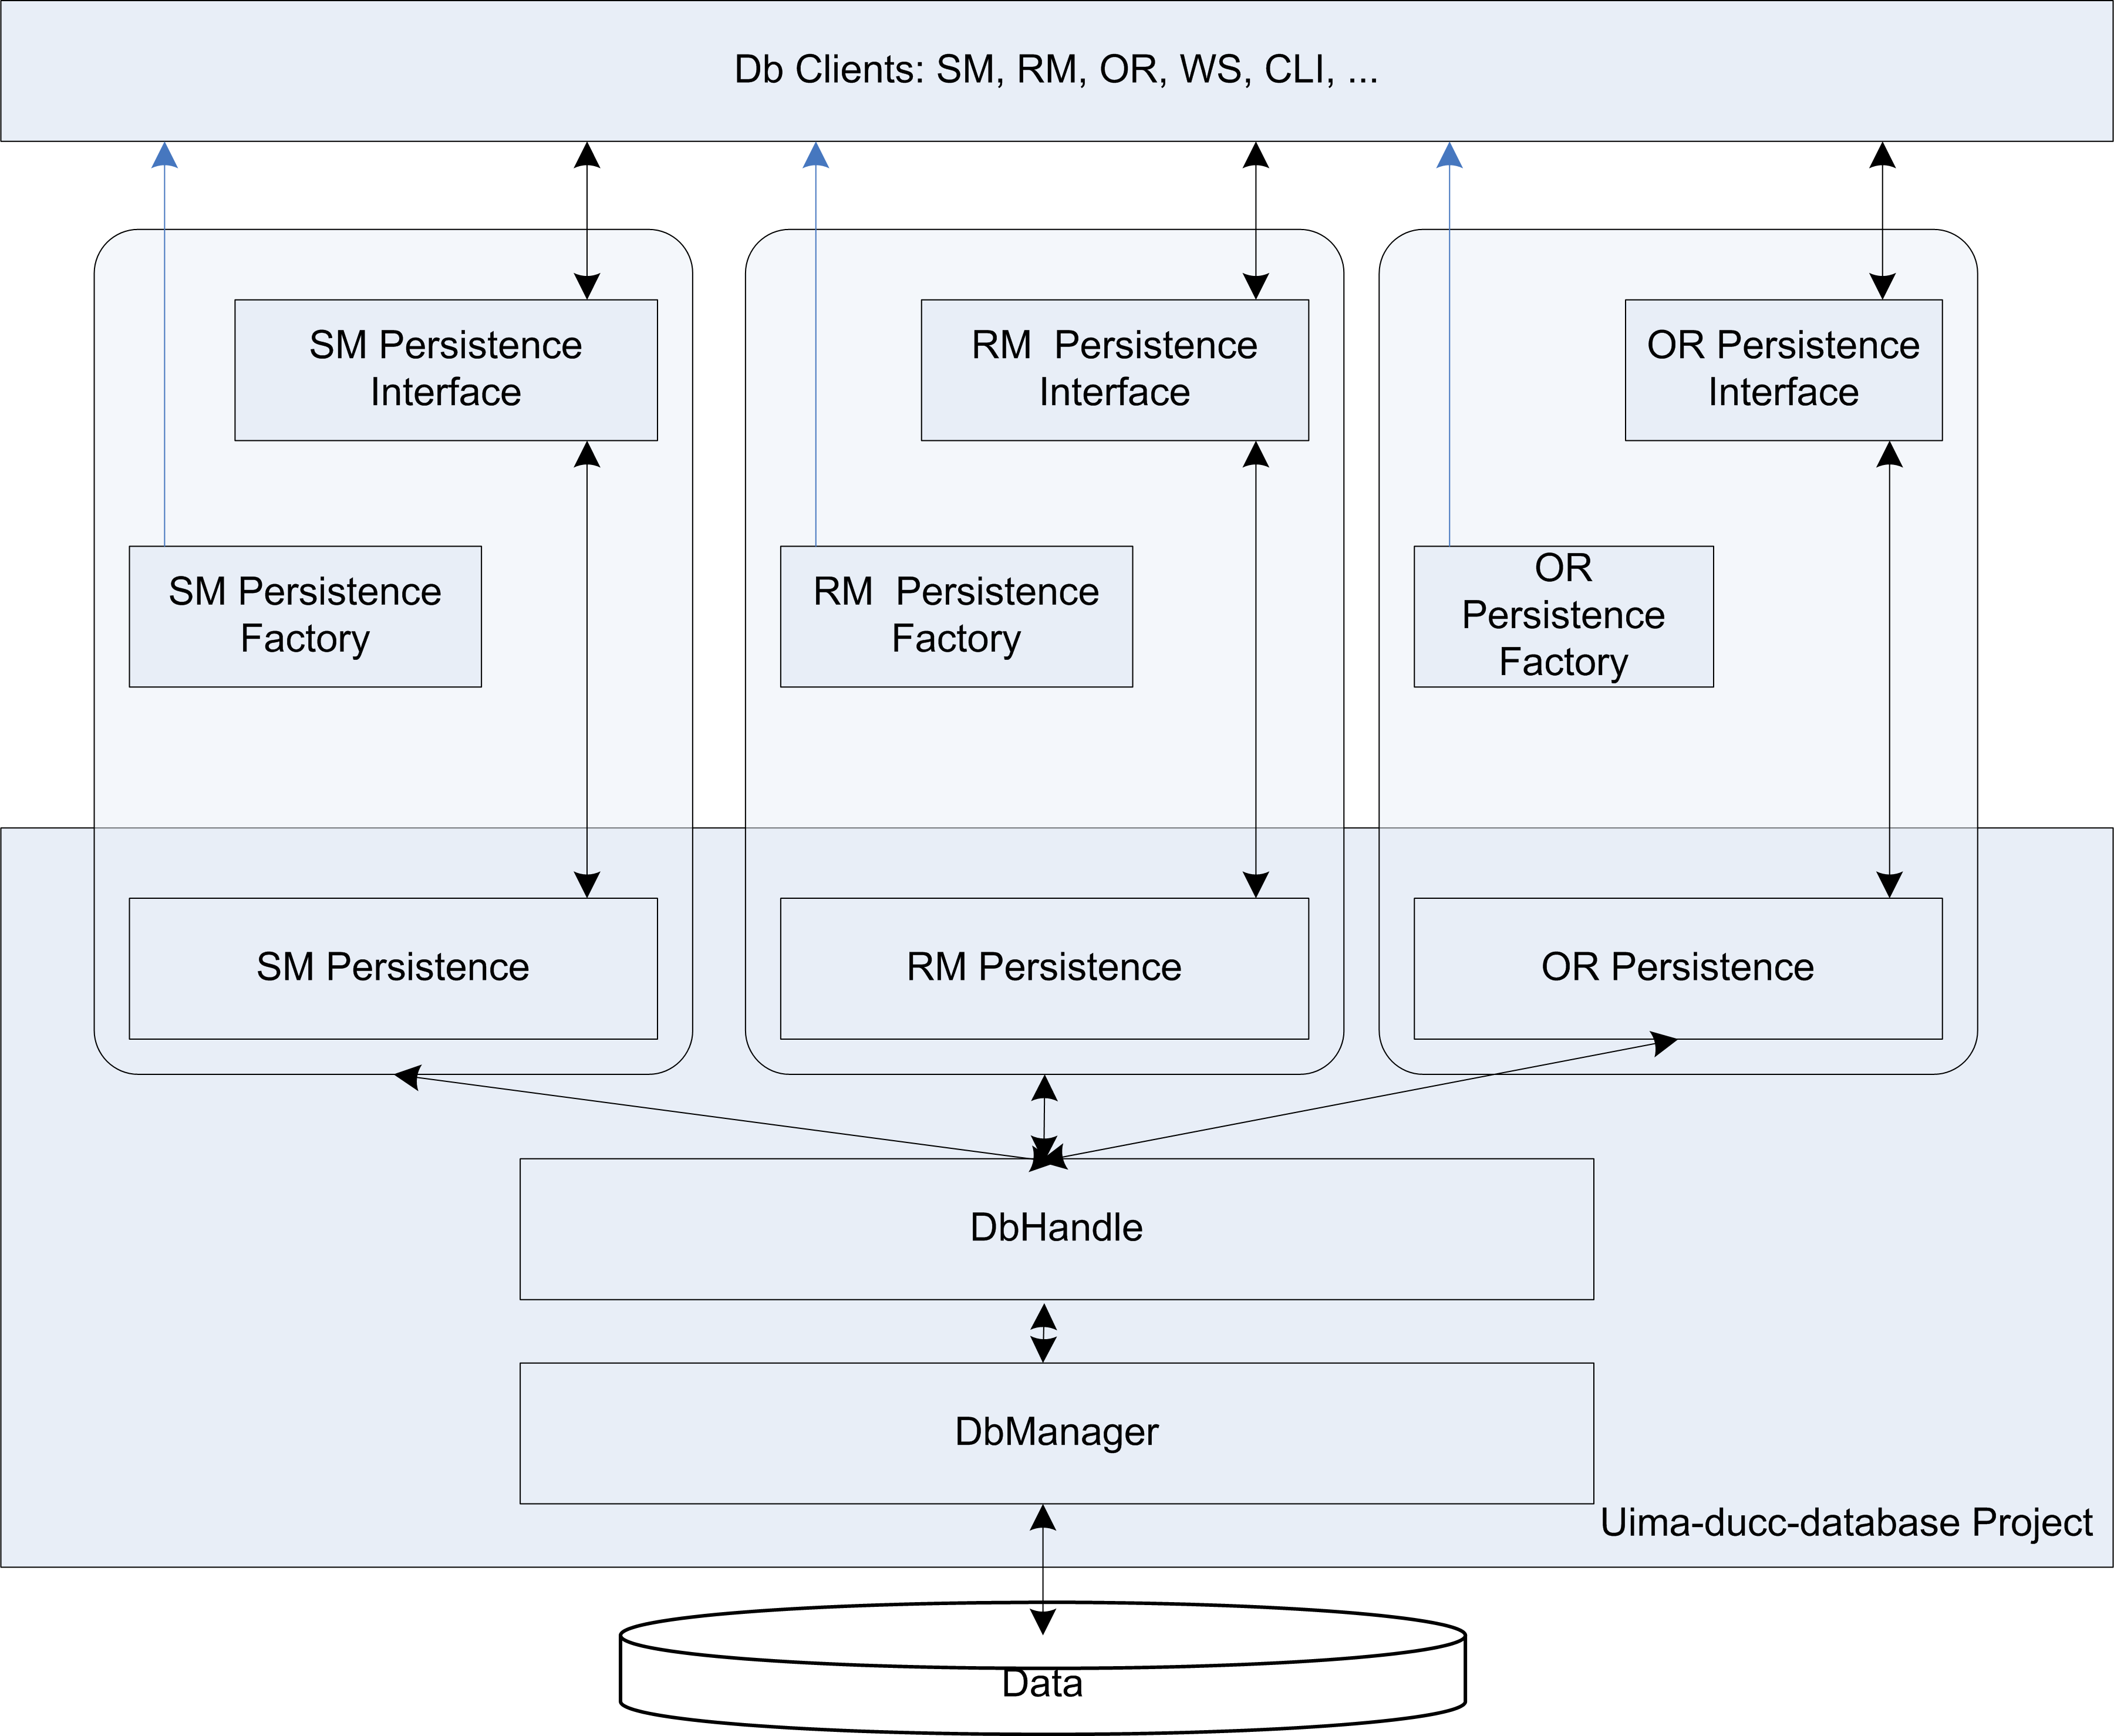
\includegraphics[width=5.5in]{images/ducc-internals/db-structure.png}
      \caption{Database Structure}
      \label{fig:db-structure}
    \end{figure}


    Runtime dependencies are resolved with reflection.  Entries in ducc.properties
    are used to specify the classes which interface with the database.  The DUCC scripting
    insures that the CLASSPATHs of components using the database contain the 
    necessary entries.

    \paragraph{Factories}
    The Cassandra Java client is thread-safe and manages connection pooling.  Only a single
    Cassandra {\em session} should be acquired for all threads in a process.  To enforce this
    the {\em Factory} pattern is used to acquire database handles.  The factory creates
    a single static handle and returns this singleton on every call.

    The objects returned by the factories are referenced through their interfaces that describe all
    legal actions against the persistent store. 

    There are three factories:
    \begin{description}
      \item[HistoryFactory.java] This resides in 
\begin{verbatim}
uima-ducc-transport/src/main/java/org/apache/uima/ducc/transport/event/common/history
\end{verbatim}
        This is used by the Orchestrator to write history files and its checkpoint, and to restore
        the checkpoint on startups.  It is used by the Web Server to read work history.
      \item[StateServicesFactory.java] This resides in 
\begin{verbatim}
uima-ducc-common/src/main/java/org/apache/uima/ducc/common/persistence/services
\end{verbatim}
        This is used by the Service Manager to maintaining service registrations, service metadata,
        and service registration history.  It is used by the Web Server to show the service
        registration and meta details.
      \item[RmPersistenceFactory.java] This resides in
\begin{verbatim}
uima-ducc-common/src/main/java/org/apache/uima/ducc/common/persistence/rm 
\end{verbatim}
        This is used by the Resource Manager to maintain its internal scheduling state for the
        purpose of inspection by other agents.  This is used by the Web Server to show machine
        details.  This is used by the admin CLI to show the state of all machines and work in the
        system.
    \end{description}
    
    \paragraph{Interfaces}
    All higher-level communication to the database is done through objects returned from the
    factories which must conform to specific interfaces.  There are three interfaces:
    
    \begin{description}
      \item[IHistoryPersistenceManager.java] This resides in 
\begin{verbatim}
uima-ducc-transport/src/main/java/org/apache/uima/ducc/transport/event/common/history
\end{verbatim}
        See its Javadoc for details of its calling sequence.
      \item[IStateServices.java] This resides in
\begin{verbatim}
uima-ducc-common/src/main/java/org/apache/uima/ducc/common/persistence/services
\end{verbatim}
      See its Javadoc for details of its calling sequence.   
      \item[IRmPersistence.java] This resides in 
\begin{verbatim}
uima-ducc-common/src/main/java/org/apache/uima/ducc/common/persistence/rm
\end{verbatim}
      See its Javadoc for details of its calling sequence.
    \end{description}

    In addition to the calling sequences, these interfaces contain Java {\em enum} structures that
    describe the database schema.  See below for how these enums are designed.

    \paragraph{Implementations}
    Multiple implementations of each interface are provided.  In all cases, a ``null''
    implementation for which all methods are empty stubs is used as a fallback in the event that a
    more functional interface cannot be provided.  There are both {\em file-based} and {\em
      database-based} implementations for Orchestrator state and for the Service registry.  Resource
    manager state is provided via the database only.  See the DuccBook for details on how to select
    a specific implementation at runtime.

    In the case of the implementations that interface with the database, an additional method is
    required, but is not part of the public interface:
\begin{verbatim}
   static RETURN-TYPE mkSchema();
\end{verbatim}
    The specific type of object returned by this method varies with database implementations.  It
    must return a collection of objects that the database creation methods can use to create the
    database schema.
    
\section{Database Schema}
    The schema for all tables is controlled by Java {\em enum} objects in the various interfaces.  These enums must adhere to a specific
    interface, defined in
\begin{verbatim}
     uima-ducc-common/src/main/java/org/apache/uima/ducc/common/persistence/IDbProperty.java
\end{verbatim}

     There are five methods defined in this interface, used by the database package to automatically generate
     the schema.  These interfaces may also be used by applications when querying the database to determine
     the types and actual database column names for each table.

     Most elements in the enum define columns of a table in the database.  Methods on the enum
     contain meta-data required to correctly create and interpret the data in a column.  Some elements in the
     enum are meta-data about the column itself.

     These methods are:
     \begin{description}
       \item[String pname()] This the name of a column as known by DUCC and may contain any ASCII
         characters.  Note this need not be the name of the column in the database.
       \item[String columnName()] This is the name of the column as used in the database.  It must
         conform to the column-naming standards of the database being used.  
       \item[Type type()] This specifies the type of data in the column.  Rather than specifying the
         database-specific type names, we supply an abstract name in the Type object which the
         database package translates to the correct form for the specific database implementation.
       \item[isPrimaryKey()] If true, the data in the column defined by this enum is a primary key.
         It is legal to specify multiple columns as primary keys, in which case, the database
         component will create a compound primary key.  The keys are generated in the order
         they occur in the enum.
       \item[boolean isPrivate()] This enum element is used by the database package only and
         should never be passed back to applications.  It allows the
         database package to maintain table-specific information that is not accidentally 
         translated into a return element. For example this is used when a row corresponds to
         a collection of Java properties, but the enum does not correspond to one of the
         returned properties.
       \item[boolean isMeta()]  This is the converse of isPrivate().  This allows
         an application to pass information to the database component that does not get
         placed into the schema or database.  For example, the name of the table may be
         defined in the enum, but this should not become the name of a column in any table.
       \item[isIndex()] If {\em true}, this column is indexed in the schema.  Multiple columns
         may be specified for indexing.
       \end{description}
     
     \paragraph{Types} We maintain a level of indirection between DUCC and specific database types, to enable
     disparate database implementation from a common meta-schema.  The DUCC-defined database
     types are:

     \begin{description}
       \item[String] The database implementation translates this into the appropriate
         type for the database, for example, {\em varchar} for a DB2 database.
       \item[Blob] This specifies a binary large object, e.g. a serialized
         Java object.
       \item[Integer] This specifies a 32-bit integer.
       \item[Long] This specifies a 64-bit integer.
       \item[Double] This specifies a Java object of type {\em double}
       \item[UUID] Some modern databases have native support for Java UUIDs.  This specifies
         an object conforming to that type.  Older databases may translate this to {\em char}
         or {\em varchar}.
     \end{description}
     
\section{The uima-ducc-database package}
     This package is intended to be isolated as much as possible from the rest of DUCC.  The
     design-point is that it should be mostly straightforward to change the database implementation,
     or to create additional persistence implementations, as long as the functions described
     in the previous sections are maintained.

     \paragraph{Database Core} Most of the database interface is contained in two classes:
     \begin{description}
       \item[DbManager] This object is responsible for directly interfacing with the
         specific database implementation.  It knows how to manage the
         database URL, how to contact the database, how to execute commands (e.g. SQL)
         against the database, how to create users and manage security, and the
         general structure of the DB API.

         This object is to be used only to initiate database communication. It generally does not
         know much about the specific query language used (e.g. CQL vs SQL), which is left to the
         DbHandle.
       \item[DbHandle] This provides a level of indirection between {\em clients} of the
         database, and the {\em implementation} of the database.  A {\em client} 
         instantiates a DbManager and then requests a {\em DbHandle} whenever it actually
         needs to communicate to the DB.  If session pooling is supported, the DbHandle should
         transparently enable this so higher-level layers need not be concerned with it.

         The handle rarely communicates directly with the database itself.  Instead, it 
         requests the DbManager that created it to do actual communication.
     \end{description}

     \paragraph{Bootstrap modules} Some specialized functions are separated into discrete classes:
     \begin{description}
       \item[DbAlive] This module communicates directly with the database, bypassing both
         the DbManager and DbHandle.  It is considered a {\em bootstrap} object.  It assumes
         the database has been started, and attempts to contact it, determine if the
         {\em ducc} and {\em guest} userids are defined, and queries the schema.  This
         implements retry logic as the database can take time to start up.  It bypasses
         the DbManager because if the database is in some way compromised, it may not be
         possible to successfully instantiate a DbManager or DbHandle.
       \item[DbCreate] This module also bypasses the DbManager and communicates directly
         with the database.  It creates the {\em ducc} superuser id, disables the
         default superuser, and creates a restricted {\em guest} userid.

         This is also considered a bootstrap object.
       \item[DbLoader] This module is used to load an existing DUCC file-based {\em history,
           checkpoint,} and {\em service registry} into the database.  It is considered a bootstrap
         module and communicates directly to the database when it can for best performance, and and
         indirectly through the implementations of the DUCC persistence objects to create summary
         tables of the various objects.
     \end{description}
     
     \paragraph{Schema Creation}
     Each of the DUCC-component-specific database implementations must implement a method
\begin{verbatim}
   static RETURN-TYPE mkSchema();
\end{verbatim}
     where the {\em RETURN-TYPE} depends on the specific database implementation.  In the case
     of Cassandra, the full signature is
\begin{verbatim}
   static List<PreparedStatement mkSchema();
\end{verbatim}

     The DUCC-component implementations inspect their schema definitions, as defined in the
     IDbProperty enums in their interfaces, and create, in the case of Cassandra, a collection
     of PreparedStatements which the {\em DbCreate} then uses to generate schema.

     \paragraph{Utility Modules}
     \begin{description}
       \item[DbUtil] This contains common, static, methods that know how to manipulate
         the IDbProperty enums to create schemas, indexes, convert property files into
         {\em INSERT / UPDATE} statements, and so on.
       \item[RmNodeState] This is example code that demonstrates one way to query the database
         and generate a {\em json} object of current Resource Manager state for clients.
       \item[RmQLoad] This is example code that demonstrates one way to query the database
         and generate a {\em json} object of current Resource Manager demand for clients.
     \end{description}
     
     \paragraph{DUCC component-specific implementations}
     These modules implement persistence for the Orchestrator, Service Manager, and Resource
     Manager, implementing their indicated interfaces as well as the required {\em mkSchema}
     methods.  They should never be directly accessed outside of the database package.  Instead,
     they must be instantiated by the correct {\em Factory} as described in earlier sections.

     \begin{description}
       \item[HistoryManagerDb]This implements persistence for Orchestrator-generated
         history and checkpoint.  
       \item[StateServicesDb] This implements persistence for the Service Manager's
         registry and history.
       \item[RmStatePersistence] This implements persistence for the Resource Manager's
         dynamic state.

         Note that this state is always deleted whenever RM initializes or reconfigures,
         and is rebuilt as the RM itself builds or recovers its dynamic state.
       \end{description}

\section{Tables}
    This section describes all of the tables.


    \paragraph{HistoryManagerDb} The {\em HistoryManagerDb} module is responsible for the
    schema and maintenance of the tables used for most of the history objects and the
    Orchestrator checkpoint.

       \begin{description}
          \item[job\_history] This contains the serialized objects for all Job history as {\em BLOB}s. 
          \item[res\_history] This contains the serialized objects for all Reservation history as {\em BLOB}s.
          \item[svc\_history] This contains the serialized objects for all Service history as {\em BLOB}s.
          \item[orckpt] This contains the Orchestrator checkpoint.  There are two {\em BLOB}s in this object:
            the current OR map, and the job-to-process map.
          \item[jobs] This contains details for all jobs, extracted from the {\em BLOB}s that are written
            to {\em job\_history}.  It does not include any process history however.
          \item[processes] This contains details for all objects that get allocated space by the RM:
            job processes, service processes, AP processes.
          \item[reservations] This contains details for all reservations, extracted from the {\em BLOB}s that are written
            to {\em res\_history}.
       \end{description}

   \paragraph{StateServicesDb} The {\em StateServicesDb} module is responsible for the 
   service registry.  

   \begin{description}
     \item[smreg] This contains the service registrations as submitted by users.
     \item[smmeta] This contains active state of services.
   \end{description}

   \paragraph{RmStatePersistence} The {\em RmStatePersistence} module is responsible for all the
   dynamic state produced by the RM.

   \begin{description}
     \item[rmnodes] This contains the state of all nodes known to the RM.
     \item[rmshares] This contains details on all the shares currently allocated by RM.
     \item[rmload] This contains the ``demand'' on the RM: counts of all services that are 
       requested by jobs, and counts of services RM is able to satisfy. (The intended purpose
       of this table is to allow external agents to inspect RM load and in conjunction with
       rmnodes and rmshares, determine whether RM is under-, over-, or sufficiently provisioned.)
   \end{description}
   
\section{Scripting and Configuration}
    The goal of the DUCC scripting support for the database is to make database start-up, shutdown,
    schema initialization, migration, and configuration as transparent as possible.  

    \paragraph{Configuration} Here we define {\em configuration} to refer to the files 
    that define the database URL, the hosts it may be running on, the
    location of the physical data, etc.  A number of these values are determined
    by virtue of the way DUCC and the database are designed to work together.  

    There are two relevant files. Pre-configured versions of these file reside in the
    DUCC source base in the directory
\begin{verbatim}
src/main/resources
\end{verbatim}

    During system build these files are copied into the database configuration
    directory.

    Note that if the database is updated or replaced it will generally be required
    to  obtain re-configure these files and replace them in the build directory.

    The files are:
    \begin{description}
      \item[cassandra.yaml] This is the primary configuration file.  Details of its
        contents are found in the standard Cassandra documentation.  We prepare this
        configuration thus:
        \begin{itemize}
          \item Set the database {\em cluster name} to DUCC.
          \item Set the hostname where the Cassandra server resides in three places:
            the {\em seed\_provider}, the {\em listen\_address}, and the {\em rpc\_address}.
            The reconfigured {\em cassandra.yaml} sets these all to the constant string
            {\em DUCCHOST}; the DUCC startup scripting changes these to the value of
            {\em ducc.head} before starting Cassandra.
          \item Set the authentication scheme to {\em PasswordAuthenticator} to force
            userid and password access.
          \item Set the authorizer module to {\em CassandraAuthorizer} to enable specific
            permissions to be set on the configured userids.
          \item Set the location of the database files in {\em data\_file\_directories}.
          \item Set the location of the database commitlog in {\em commitlog\_directory}.
          \item Set the location of the database saved caches in {\em saved\_caches\_directory}.
        \end{itemize}
      \item[cassandra.env.sh] This is a shell script that is run by Cassandra as it is
        starting up to detect the environment and set its internal parameters. The following
        DUCC changes are applied:
        \begin{itemize}
          \item Alter checks for the JVM vendor so it will start with the IBM JVM.
          \item Parameterize some things so the can be pulled from the environment, and
            thus enable Cassandra to be customized from {\em ducc.properties}.  The following
            items have been modified in this file for this purpose: JMX\_PORT.  (Note that
            {\em Xmx and Xms} are already customizable by setting environment variables.)
        \end{itemize}
      \end{description}
    
      \paragraph{Scripting}
      
      
      \paragraph{} 

      The following updates to the DUCC scripting support the database:
      \begin{description}
         \item[ducc.head Configuration] When DUCC is started, a small bit of code is executed to insure
           the {\em ducc.head} node is properly configured in the Cassandra configuration {\em
             cassandra.yaml}.  If not, a message is emitted and the configuration file is updated
           before attempting to start DUCC.
        \item[ducc\_util.py] This contains common database routines used by all scripts that extend
          the base class {\em DuccUtil}.  These methods perform these functions:
          \begin{description}
            \item[Enable DB] db\_configure reads {\em ducc.database.host} and if it is set to
              ``--disabled--'', a global variable is set to indicate the DB is disabled.  Otherwise
              it reads the database password from {\em ducc.private.properties} and sets that into
              a global variable.  If there is no password set, the DB is set disabled regardless of
              the value of {\em ducc.database.host}.
           \item[DB process running] db\_process\_alive attempts to determine if the database process
             is running (which is not equivalent to the database being functional).
           \item[DB functional] db\_alive attempts to contact the database by calling the Java bootstrap
             routine ``DbAlive'' (see previous section).  It returns true or false to indicate whether
             the DB appears functional.
           \item[DB stop] db\_stop uses the Cassandra pid to send {\em kill -TERM} to stop the DB process.
           \end{description}
         \item[db\_util.py] This contains database methods that can be called from any scripting that
            need not extend {\em DuccUtil}.  It contains methods to stop the database, update 
            {\em cassandra.yaml} with the value of {\em ducc.head}, and assist parsing and formatting
            the results of executing {\em cqlsh}.
          \item[ducc.py] This contains a method to start Cassandra.  It is called from {\em start\_ducc}
            and {\em startsim}.
          \item[start\_ducc] This contains calls to {\em ducc\_util.py}  and {\em ducc.py} to configure
            and start the DB, and then insure it comes up before starting the rest of DUCC.
          \item[stop\_ducc] This contains calls to {\em ducc\_util.py} to stop the DB.
          \item[check\_ducc] This contains calls to {\em ducc\_util.py} to determine if the DB is running or not.
          \item[ducc\_post\_install] This contains calls to {\em db\_util.py} to configure the
            {\em ducc.head}, generate a random database password, and initialize the schema.
          \item[db\_create] This contains methods to define a database, independently of
            {\em ducc\_post\_install} intended for migration purposes.
          \item[db\_loader] This contains calls to the java utility {\em DbLoader} to
            migrate existing state and history files to the database.
          \item[startsim] This contains calls to {\em ducc\_util.y} to start the database and
            insure it starts correctly.
          \item[stop\_sim] This contains calls to {\em ducc\_util.y} to stop the databse.
          \end{description}
          



\chapter{Resource Manager}
% 
% Licensed to the Apache Software Foundation (ASF) under one
% or more contributor license agreements.  See the NOTICE file
% distributed with this work for additional information
% regarding copyright ownership.  The ASF licenses this file
% to you under the Apache License, Version 2.0 (the
% "License"); you may not use this file except in compliance
% with the License.  You may obtain a copy of the License at
% 
%   http://www.apache.org/licenses/LICENSE-2.0
% 
% Unless required by applicable law or agreed to in writing,
% software distributed under the License is distributed on an
% "AS IS" BASIS, WITHOUT WARRANTIES OR CONDITIONS OF ANY
% KIND, either express or implied.  See the License for the
% specific language governing permissions and limitations
% under the License.
% 


This chapter provides architectural and implementation details for the DUCC
Resource Manager, referred to as the ``RM''.
\section{Introduction}

The DUCC Resource Manager is responsible for apportioning cluster resources to the
collection of ``work'' to be run by users.  Work is classified into several categories.  As
exposed in the public interface, these categories are:

\begin{description}
  \item[Fair-Share Job] This is a UIMA/AS job, consisting of a minimum of two processes and 
    a potential maximum of as many processes as physically fit on a cluster.  The work
    executed by the processes is parallel, enabling the RM to expand or contract
    the job by allocating or deallocating processes as needed to balance the load.

    Load is balanced using a weighted fair-share policy in which all users are apportioned an
    equitable amount of the cluster resources, where ``cluster resources'' refers only to real
    memory on the cluster nodes.

  \item[Service Instance] This is any arbitrary process that DUCC manages as a ``service''.
    Services are registered with the Service Manager and may be comprised of multiple physical
    processes.  (See the DuccBook for details of DUCC Service Management.)  The RM schedules these
    processes as singletons, using a non-preemptive policy (FIXED\_SHARE or RESERVE).

  \item[Arbitrary Process or ``Managed Reservation''] These are singleton processes of any type, scheduled
    using a FIXED\_SHARE policy.

  \item[Fixed-Share Job] This is a UIMA-AS job scheduled with a non-preemptable, i.e. FIXED\_SHARE
    policy.

  \item[Reservation] This is a request for a dedicated full machine.
\end{description}

The RM is a memory scheduler only.  The use case which justifies DUCC is UIMA-AS jobs, each of
which consists a variable number of parallel processes, each of which requires large amounts of memory, usually
on the order of 16GB or more.  Memory requirements completely overwhelm other resource
requirements, so that jobs scheduled by their declared memory sizes usually get sufficient
other resource such as CPU. 

\section{Vocabulary}
    In order to understand RM it is necessary to understand some of the language used in RM.

    \begin{description}
    \item[quantum] This is the smallest memory size of an allocation, defined in multiples of GB.  It
      is defined globally in {\em ducc.properties} and may be overridden in {\em ducc.classes} for
      top-level nodepools.  See the DuccBook for more details.
      
      Note that although DUCC defines a quantum, most of the RM does not
      use quantum at all; instead it generalizes quantum into {\em qshare}, {\em nshare},
      and {\em order} as defined below.  When a schedule is returned to the Orchestrator, the
      allocations, in terms of quanta, are translated back to memory allocations using this
      configured {\em quantum}.
      
    \item[qshare] This is an abstract memory allocation representing exactly one {\em quantum}.  Memory
      allocations are made in terms of some multiple of {\em qshares}.

    \item[nshare] This is an allocation which consists of one or more co-located {\em qshares}.  When 
      exposed outside of RM this is usually thought of as a ``process''.  It means, literally,
      ``n qshares''.  
      
        Be careful, an {\em nshare} is NOT a process, it is an allocation that can be put to
        any use or to no use if desired.  The RM does not care what an {\em nshare} is used for.

      \item[order] This is a number which refers to the number of {\em qshares} associated with some
        entity such as a machine, a job, a process, an {\em nshare}.  An ``order 3'' machine is a
        machine whose memory can be counted as ``three qshares''.  An ``order 3'' job is a job whose
        processes must be allocated as ``three qshares'' each, or one ``order three'' nshare.

        All {\em qshares} are of order 1, but we don't know how much that is without knowing
        the {\em quantum}.  

        {\em Order} is an abstraction of the {\em quantum}.  Knowing the {\em order}
        of any entity does not tell one how large that entity is.  It does tell one
        how big that entity is in relation to other entities.

        Note that {\em order} is NOT an allocation; it is not a {\em qshare} or an {\em nshare}.
        It is a number which describes the size of things, without saying how big that size
        is or what that thing is.

        Order is used throughout the RM to index arrays and is one of the most fundamental
        concepts in the RM architecture.
      \end{description}
      
\section{Architectural Overview}
    Throughout this section, please refer to the diagram in \hyperref[fig:rm-structure]{Figure ~\ref{fig:rm-structure}}.
    The diagram shows the normal flow through the scheduler, from the time and Orchestrator
    publication arrives to the time the RM publishes its schedule.

\subsection{The Onion}
    At the highest level of abstraction, the RM consists of three layers as seen in the 
    \hyperref[fig:rm-structure]{Figure ~\ref{fig:rm-structure}} below.  It can be thought of as a three-layer onion:
    \begin{description}
    \item[JobManagerConverter] This is the outer layer.  This layer communicates with the
      ``outside'' world: the DUCC Orchestrator and DUCC agents.  It is conceived of as in
      ``impedance matcher'' that converts incoming messages to the RM's internal structures, and
      converts the RM's internal structures into structures recognized by the outside world (the
      DUCC Orchestrator). It is possible to replace this layer without affecting the RM proper; for
      example, to create an isolated simulator for RM development.
    \item[Scheduler] This is the middle layer.  It communicates on one hand with the {\em JobManagerConverter}
      to receive and send data outside of RM and on the other, with the inner layer, the {\em NodepoolScheduler}.
     \item[NodepoolSchedler] This is the inner layer and is the ``scheduler proper''.  Its input is
       a set of allocation requests and its output is a set of node assignments for each request.  These are
       passed up through the {\em Scheduler} and again up to the {\em JobManagerConverter} for publication.
    \end{description}
    
\subsection{Nodes, Machines,  and Node Management}
    The resources scheduled against are nodes.  On each physical node is a DUCC Agent which
    publishes a regular ``heartbeat''.  The ``heartbeat'' contains data describing the
    characteristics of the node used for scheduling: the memory size, the node name, the 
    node IP.  

    If a node fails, its ``heartbeat'' stops arriving.  After some number of missed
    heartbeats, the RM considers the node to be unusable; it will stop scheduling work
    to that node and attempt to evict existing work from the node.  Work that can
    be rescheduled (fair-share jobs and services) get rescheduled on working nodes.

    It is possible to remove a node from scheduling without the node failing using the
    {\em vary\_off} utility.  This causes the RM to stop scheduling work to the 
    specified node, and it causes fair-share work to be evicted and rescheduled elsewhere.

    The RM component responsible for managing nodes is {\em NodePool.java}.  As each
    node heartbeat arrives, the {\em NodePool} is notified and, if it is the first
    such notification, creates an object RM calls the {\em Machine} to represent the
    remote resource.

    The RM implements multiple nodepools in a nested or tree structure.  There is one NodePool
    object for each configured nodepool.  The NodePools are structured in a self-organizing
    tree (that is, none of the Java collection classes are used to organize multiple nodepools).
    Most of the methods inside the NodePool module are recursive, aware of their parent
    NodePools and child NodePools.

\subsection{Jobs}
    The RM is mostly unaware of the purpose for which allocations are made.  It uses a
    single structure, the {\em RmJob} to represent all work.  There are a small number
    of minor switches in the code in deference to specific types of work (UIMA-AS jobs
    vs reservations, for example) but these are not sufficient to justify a more elaborate
    object structure.

\subsection{Shares and share-order}
    All RM allocations are in terms of {\em shares}. A share represents some portion
    of the real memory on a node.  The smallest {\em share} than can be allocated is
    called a {\em quantum share}.  The size of the {\em share quantum} is declared
    in {\em ducc.properties} and can be overridden for {\em top-level nodepools} in
    {\em ducc.classes} (see the DuccBook for the details of quantum configuration).

    In the RM, a single quantum share is called a {\em Qshare}.  Multiple co-located {\em qshares}
    may be allocated for any given request.  A multi-qshare allocation is called an {\em nshare}. A
    {\em nshare} always corresponds to 
    \begin{itemize}
      \item A single process of a FAIR\_SHARE job,
      \item A single process of a FIXED\_SHARE job,
      \item A single service instance process,
      \item A single AP (or ``managed reservation'',
      \item A single unchanged reservation.
    \end{itemize}

    Thus a job may be allocated multiple {\em nshares}.  {\em Nshares} are usually exposed outside
    of RM under the term {\em process}.  (There is a difference: an {\em nshare} refers to an
    abstract allocation; a {\em process} refers to some physical process running on a node.  RM only
    needs to deal in abstractions.)
    
    The term {\em share-order} is used to refer to the number of {\em qshares} associated with
    an entity.  Entities with associated {\em share-order} include
    \begin{itemize}
      \item Jobs.  The {\em share-order} of a job is the number of {\em qshares} required
        to make a single {\em nshare}.  It is a translation of the job's declared memory
        requirements into the number of share quanta required per process.
      \item Nodes (Machines).  The {\em share-order} of a machine is the number of
        {\em qshares} that can be allocated on that machine.  It is a translation of the
        machine's real memory into the number of share quanta that can be allocated to the machine.
      \item Shares.  The order of a {\em share} is the number of {\em qshares} represented
        by the {\em Share} object.  Note this implies that a {\em Share} object always
        represents a single {\em Nshare}.
    \end{itemize}
    
    All of the important algorithms in the RM involve managing incoming work and
    resources by their ``order''.

    A Job's memory specification are converted to {\em share-order} thus:
\begin{verbatim}
    share_order = job_declared_memory / share_quantum
    if ( job_declared_memory % share_quantum ) > 0
        share_order + share_order + 1
\end{verbatim}
    Note that a job's share order is always rounded UP.    
    
    A Machine's announced memory is converted to {\em share-order} thus:
\begin{verbatim}
    share_order = (int) (allocatable_mem / share_quantum;
\end{verbatim}
    Note that a machine's share order is always rounded DOWN.

\subsection{Users}
    Every job that arrives has an associated user.  The RM maintains a map of all users and
    maintains a two-way map of jobs-to-users.  Note that every job has exactly one {\em user} 
    but that every user may have an arbitrary number of {\em jobs}.  Thus, a user may
    be associated with work of different {\em order}s and running in different {\em classes}
    under differing policies.  The structure defined in {\em User.java} maintains all
    necessary records as used by the scheduler.

\subsection{RM Structure Schematic}
    \begin{figure}[H]
      \centering
      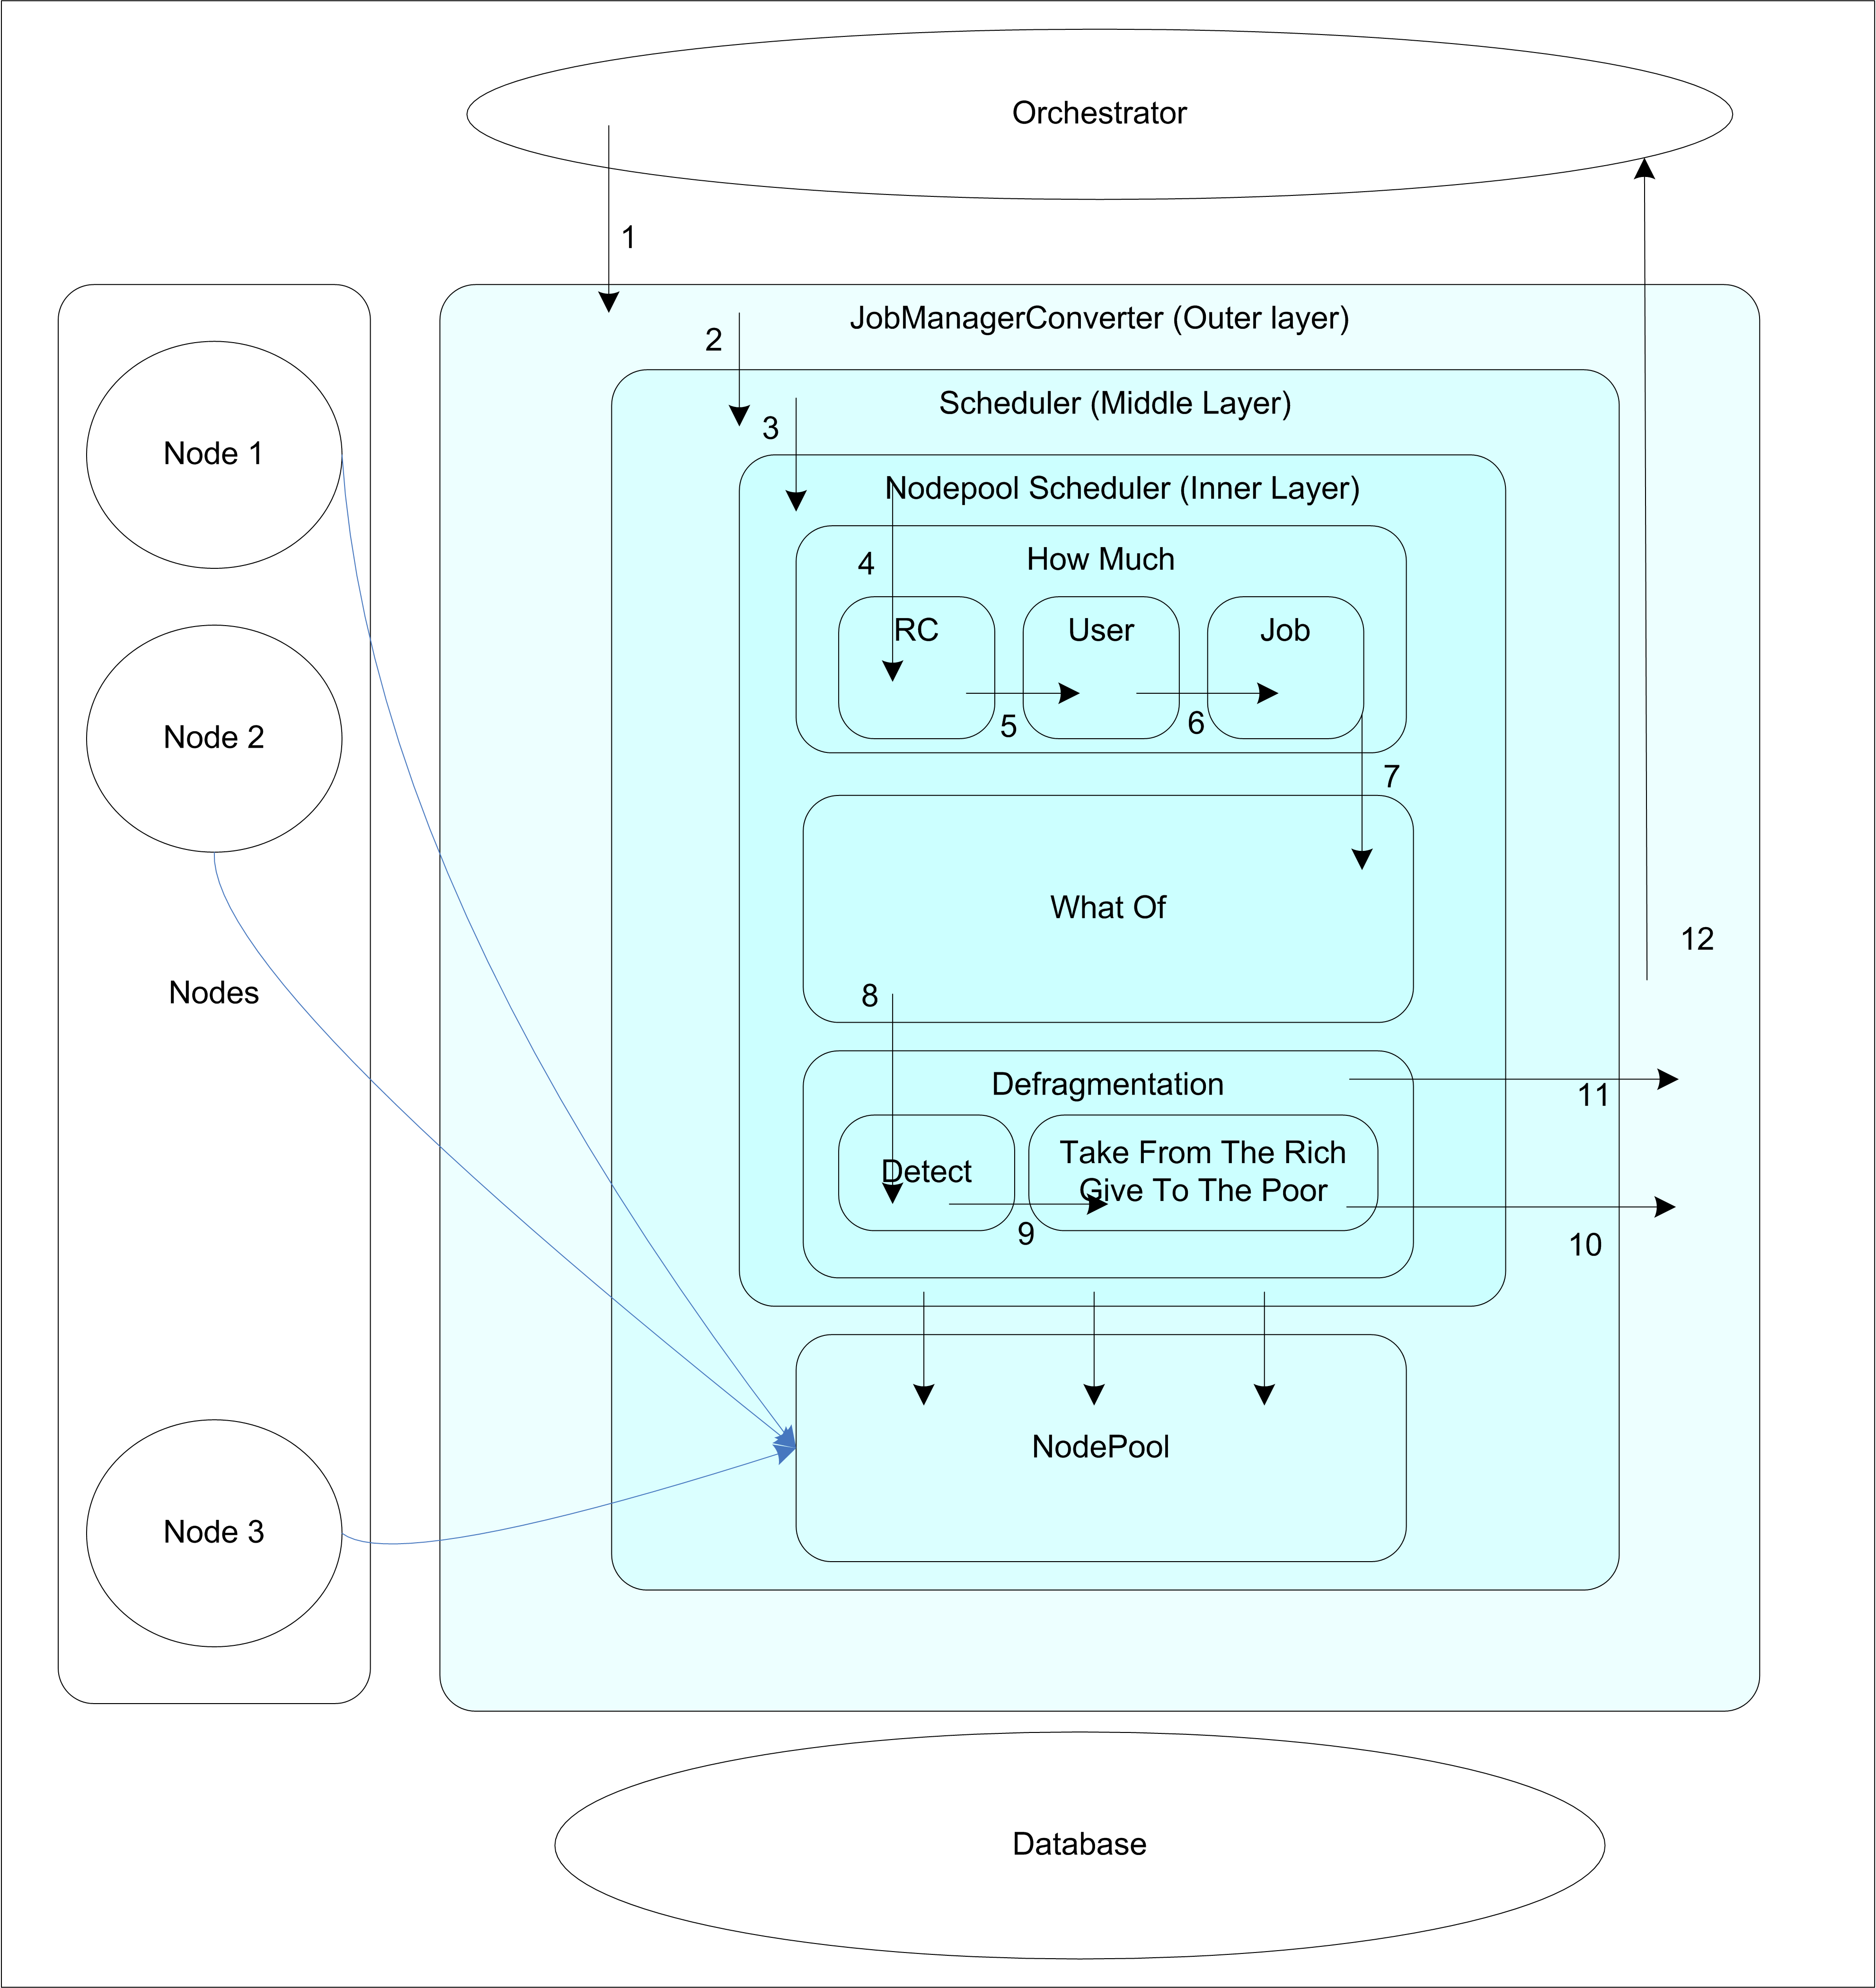
\includegraphics[width=5.5in]{images/ducc-internals/rm-structure.png}
      \caption{RM Structure}
      \label{fig:rm-structure}
    \end{figure}

\section{Outer Layer: JobManagerConverter}

    The {\em JobManagerConverter} is the outermost layer of the RM.  It is intended as a
    buffer or ``impedance matcher'' to protect the RM from the ``outside world''.  It is
    also intended to be replaceable as needed. It communicates with the middle layer through
    an interface.   Any entity that (correctly) uses this interface may act as the outer layer.

    This section describes the most important
    functions of the {\em JobManagerConverter} in detail.  We refer to this as the 
    JMC for brevity.

    The primary function of the JMC is to receive incoming work in the form of Orchestrator
    publications and convert them into a set of discrete scheduling events to be passed to the inner
    layers of the RM.

\subsection{Incoming Work}
    Key methods involved in receiving work and passing it to the next layer are described here.

    \paragraph{eventArrives()} receives the {\em DuccWorkMap} from the Orchestrator.  

     If the RM is not yet initialized the map is ignored.

     If the RM has been recently reconfigured, all structures in JMC are cleared and 
     state set as if this is the first publication.

     If this is the first publication, we pass the map to the method {\em recoverFromOrchestrator}
     to initialize essential structures for work that has {\em ALREADY} been scheduled and is
     running in other parts of the system.  This step is needed for these cases:
     \begin{itemize}
       \item DUCC is being started ``warm''.  In this case the Orchestrator map may include
         Reservations, which are permanently scheduled, and must be recovered. 
       \item The RM may have been stopped (or crashed) and is being restarted.  In this case
         work of all sorts that was already scheduling must be recovered.
       \item The RM may have been dynamically reconfigured.  Dynamic reconfiguration requires
         that all internal structures be reset.  This is the equivalent to stopping and then
         restarting the RM.  Work must be recovered.
     \end{itemize}
     
     The incoming map is now saved for the map-difference code.  If this is the first publication,
     RM simply returns.

     All subsequent Orchestrator publications are compared with the previous map and
     all differences are converted to scheduling events. 

     There are three types of events:
     \begin{description}
       \item[New work] If the work has never been seen before, it is passed to the method
         {\em jobArrives} for conversion into the RM internal structure {\em RmJob}.  The new
         work is passed to the middle layer {\em Scheduler} via {\em signalNewWork()}.
       \item[Completed Work] If the work is marked {\em completed} by the Orchestrator it is
         removed from the local map and the {\em Scheduler} is signalled via {\em signalCompletion()}.
       \item[Existing Work] The associated {\em process map} for each DuccWork object is differenced against the
         previous map to identify processes which may have
         completed or otherwise changed state.  The {\em RmJob} is fetched from {\em Scheduler} and
         the state of its shares or the job itself is updated.  If a process is completed,
         the {\em Scheduler} is signalled via {\em signalCompletion()}, overloaded on share instead of job.  If
         at least one process has reached the {\em Running} state the {\em RmJob} is notified so
         the {\em expand-by-doubling} policy can be enacted.
     \end{description}

     Once the incoming events are processed the middle layer is signaled by invoking the method
     {\em schedule()}.

\subsection{Outgoing Events}
     A schedule is returned from {\em Scheduler} in the form of a {\em JobManagerUpdate} object.  This
     object must be translated into an outgoing publication of the form expected by the Orchestrator.  The
     {\em JobManagerUpdate} is passed to the {\em JobManagerConvert.createState()} method for conversion.

     The final publication is returned in the form of a {\em RmStateDuccEvent} which is then passed to the
     Camel framework for publication.

\section{Middle Layer: Scheduler}

    The ``middle layer'' is implemented in {\em Scheduler.java}.  This entity must conform to the
    interface {\em ISchedulerMain} to maintain the layered ``onion'' architecture.  The ``outer layer''
    does all its interactions with the scheduler proper through this interface.

    The middle layer is relatively straightforward.  It is the middle-man between the {\em JobManagerConverter}
    and scheduler proper, responsible for initialization, global bookkeeping, and dispatching of events
    to the correct objects.  We'll simply list the important functions
    and how to find them:

    \begin{description}
      \item[Initialization] {\em Scheduler.init()} is called from the DUCC infrastructure for RM,
        {\em ResourceManagerComponent}.  RM configuration from {\em ducc.properties} is loaded, the
        class configuration from {\em ducc.classes} is loaded, the RM configuration is announced to the
        log, the database of dynamic RM data is cleared, and the ``initialized'' flag is set to ``true''.
      \item[Class configuration] This ({\em initClasses()}) is invoked out of {\em init()}.  The class configuration is loaded
        into the common {\em NodeConfiguration} object and a set of {\em ResourceClass} objects is
        created.  The {\em NodePool} objects are instantiated.
      \item[Re-configuration] This is implemented in the {\em reconfigure()} method.  Most internal structures
        are cleared and released and {\em init()} invoked as described above.
      \item[Node Publications] All node publications are passed to the method {\em nodeArrives()}. This
        method does a bit of bookkeeping, works out the {\em order} of the node, records the {\em node heartbeat},
        and passes the node to its NodePool for future scheduling.
      \item[Run Scheduler] The {\em schedule()} method is invoked from the outer layer as described
        in the previous section.  This method drains incoming events, ``recovers'' any
        previously-scheduled work, updates state to reflect processes which have exited, and enters
        new jobs and users into the system.  It then invokes the ``inner layer'', the {\em
          NodePoolScheduler} on each top-level nodepool.  This results in creation of the new
        schedule which is passed back to the outer-layer for publication by means of the {\em
          dispatch()} method.
      \item[Dispatch] This method ({\em dispatch()}) records the current schedule in the log
        and converts the schedule into a form usable by the {\em JobManagerConverter} for publication. The
        object created here, {\em JobManagerUpdate} is passed up and published.
      \item[CLI] All CLI methods are handled here, passed in from the outer layer from {\em ResourceManagerComponent}.
        
    \end{description}

\section{Inner Layer: NodepoolScheduler and NodePool}
   The {\em NodePoolScheduler} and it's helper {\em NodePool} comprise the ``scheduler proper''.  They are
   both relatively complex.  This section discusses their architecture and the general flow of data
   through them.  Readers would be advised to have code listings handy if the goal is to fully understand
   the DUCC Scheduler.

   The {\em NodepoolScheduler} is the ``main'' scheduler.  An analogy would be that it is the ``frontal cortex''
   of the brain, doing most of the abstract reasoning required to form a schedule.

   The {\em NodePool} is a helper class, responsible for managing physical layout of processes ({\em ``nshares''})
   over physical nodes ({\em Machines}).  It can be thought of as the ``cerebellum'', controlling the ``arms and legs''
   of the schedule.

    The scheduling rule {\em ``priority''} is implemented by executing the {\em How Much} and {\em
      What Of} phases once for each priority, starting with the ``best'' priority, down to the
    ``worst'' priority.  At each stage the scheduler attempts to give away all of its
    resources. Each subsequent cycle through this loop will generally have fewer resources to
    allocate until either all work is scheduled, or all resources are exhausted, whichever comes
    first.

    After the first two phases are complete in all passes, all fair-share jobs are iterated and any job whose
    physical allocation exceeds the number of resources counted in the ``How Much'' phase has its surplus
    processes preempted.  (These preempted resources are NOT added back to the resource pools until the Orchestrator
    confirms they have exited; hence they aren't accounted for in the ``what of'' phase AT THIS POINT. They
    will be used once they are known to be free.)

    Finally, the {\em defragmentation} phase is executed.

\subsection{NodepoolScheduler}

    We will use a ``divide and conquer'' approach to describe the {\em NodpoolScheduler}.  This component consist of
    three primary parts:
    \begin{description}
      \item[How Much.]  This phase performs the FAIR\_SHARE calculations as well as works out the
        allotments for FIXED\_SHARE and RESERVE requests.  It assumes an ``ideal'' configuration of
        nodes with no conflicts and no fragmentation.  There is one {\em How Much} method for
        each of the three scheduling policies ({\em howMuchFairShare(), howMuchFixed(),} and
        {\em howMuchReserve()}.
          

      \item[What Of.] This phase works closely with the {\em NodePool} to try to find available
        space for the abstract allocations produced by the ``How Much'' phase.  It is responsible for initiating
        preemptions but it never preempts a job below the counts from the ``How Much'' phase.  It preserves
        a stable layout by never preempting work that is already allocated unless that work is exceeds
        some user's fair share as determined by the ``counts'' from ``How Much''.
        
        Note that because it is constrained by the existing layout it may not always succeed
        laying out all work.  If this occurs we must perform ``Defragmentation''.

        The three relevant methods are {\em whatOfFairShare(), whatOfFixed(),} and {\em whatOfReserve()}.

      \item[Defragmentation] After ``What Of'', a pass is made to insure that every job is allocated
        its fair share.  If not, defragmentation is performed to insure that at least ``some minimum'' 
        number of processes is allocated for every job.  This may involve preemptions
        of job processes even for user whose allocations are at or below their fair share.
    \end{description}


    We now describe these three actions in detail.

\subsubsection{How Much}

    For non-preemptive work this is straightforward: the work is assigned whatever is asked for UP TO
    the configured user allotment (see the DuccBook for details of allotment).  Non-preemptive work 
    belonging to users who are at or over their allotment is deferred and not passed to further scheduling stages.

    The FAIR\_SHARE algorithm is performed on each of three {\em entities}: The ResourceClass, the User, and
    the RmJob.  Throughout the rest of the discussion the term {\em entity} is used to refer to any
    of these when the specific type of object is not relevant.  (Each of these entities implement the
    generalized {\em IEntity} interface.).

    \begin{description}
      \item[ResourceClass] Every {\em ResourceClass} is asked to provide a summary of how many {\em nshares}
        of each size it could use, assuming unbounded resources, (but constrained by RM rules such
        as initialization cap and expand-by-doubling).  They produce an
        array, indexed by {\em share order} of the number of processes of each order they want allocated.

        To produce this array, the {\em ResourceClass} iterates all jobs ({\em RmJob} structures) assigned to the class and ask 
        the same question of the RmJobs:, ``in an unbounded world what is the maximum number of processes you require''.  The
        method responding, {\em RmJob.getJobCaps()} examines the number of work items not-completed, the number
        of threads per process, and their {\em process\_deployments\_max} to produce an initial guess.  It then
        takes into account ``doubling'' to revise the estimate down.  It then uses the process initialization
        time and average execution time per work-item to again revise the estimate down if it appears
        new allocations would not be used by the time they were made available. (This process is described in greater
        detail below.)

        The short description of what {\em getJobCaps()} does is this: start with the largest reasonable request
        and whittle it down using the constraints of the RM rules to the smallest number of processes that
        is guaranteed to be used, RIGHT NOW.

        The sum of all job caps by ResourceClass, indexed by {\em share\_order} is used to create
        the scheduling {\em demand.}
        
        The NodePools are then interrogated to produce a similar array, indexed by {\em share
          order}, of the number of processes they can provide, accounting only for existing
        committed allocations This produced an idealized view of the {\em resources}.

        The algorithm implemented in {\em apportionQShares} then performs a FAIR\_SHARE allocation of
        {\em nshares} to every job by matching {\em demand} with {\em resources}. We'll describe this allocation in greater detail below.

        At the end of this phase, every {\em ResourceClass} contains a table called {\em given\_by\_order} which is 
        the number of {\em nshares} indexed by {\em share order} to be assigned the jobs in the ResourceClass,
        according to weighted fair-share.  At this stage
        it is not known if it is physically possible to actually fulfill these allocations.

      \item[User] Next, for each resource class, all the users owning jobs in that class are
        gathered.  The same weighted FAIR\_SHARE code is executed against users, counting only jobs
        in the current class, but using the hard-coded weight of ``1'' (one).  This results in an
        equitable distribution of the weighted FAIR\_SHARE allocations from the current ResourceClass among
        the users of that class.

        At the end of this phase, every {\em User} contains a table {\em given\_by\_order} which is the total
        shares allocated to this user, for all jobs in this class.

      \item[Job] After allocating jobs among users for each resource class, each {\em User} with
        jobs in the class has the shares apportioned by the previous steps divided equally among all
        their jobs in that class, again using the same weighted FAIR\_SHARE routine with hard-coded
        weight of ``1'' (one).

        At the end of this phase as before, all affected {\em RmJob}s have a table {\em
          given\_by\_order} which contains the number of {\em nshares} assigned to that
        job.
    \end{description}

\subsubsection{apportionQSares()}    
    The method {\em apportionQShares()} is the method that performs the FAIR\_SHARE allocation for the
    ``How Much'' phase.

    The {\em apportionQshares()} method is much more involved than simply performing a weighted apportionment
    of some abstract number of qshares among the various entities (ResourceClass, User, RmJob).  Because
    every resource may be of different {\em share order}, and the set of jobs being scheduled to a ResourceClass
    are generally of  different {\em share order}, this method must perform an equitable distribution of {\em qshares} but it
    must assign them as {\em nshares} that can be also physically allocated.  We must perform weighted fair-share
    against the ``demand'' in terms of basic scheduling unit {\em qshares}, but we must produce a tentative schedule in terms of
    {\em nshares} which can be mapped to real, known, physical machines.

    State simply, it is useless to allocate shares on a machine of order $n$ to a job of order $>n$: the
    job won't ``fit''.

    In {\em apportionQShares()} we perform a series of iterations by decreasing {\em share\_order},
    each iteration performing ``fair share'' allocation of resources among resources of that order,
    but using the TOTAL demand in {\em qshares} of the entity, ignoring for the moment whether it
    will ``fit''.

    At the end of each iteration, entities which have their ``demand'' satisfied at the current
    order are removed, and the iteration is repeated with the next smaller order, until either all
    ``demand'' is satisfied or all resources are exhausted.

    This produces an imperfect schedule that is ``pretty close'' and is computationally simple to
    produce.  The defragmentation step at the end of scheduling provides additional correction.

    The general mechanism is as follows:
    \begin{itemize}
      \item Initialize the {\em wanted\_by\_order} structure (the number of {\em nshares} of each {\em share order}
        wanted by all entities in the current pass.
      \item Starting at the largest share order, called ``current order'',
        \begin{itemize}
          \item Calculate weighted FAIR\_SHARE for only entities of ``current order'' against all resources of
            current order or greater, using total unfulfilled {\em demand} for the entity.
          \item Assign new {\em nshares} to the entities, incrementing their {\em given\_by\_order} for the current order.
          \item Decrement entities' {\em wanted\_by\_order} (i.e., their {\em demand}.)
          \item Remove all entities whose total allocation has been satisfied.
          \item Decrement the ``current order'' and repeat.
        \end{itemize}
      \item If any {\em wanted\_by\_order} has non-zero entries, repeat this entire procedure until either all of {\em wanted\_by\_order}
        becomes zero, or until no more resources are assigned (meaning they have been exhausted).
      \end{itemize}

      After this phase has been executed for every entity, every {\em RmJob} has a table of
      ``counts'' which indicates the number of processes to be allocated to it.

\subsubsection{What Of}

  The {\em What Of} phase attempts to find physical resources to match the ``counts'' from ``How Much''.  Note
  that we no longer deal with Users.  We use ResourceClasses in this phase ONLY to find the correct
  NodePool.  The RmJob is the focal point of ``What Of''.
  
  The general mechanism is the same for all types of allocations at this point: collect all jobs
  for each resource class, and ask the NodePool assigned to that class to find ``open'' spots
  of the right size for every counted {\em nshare}.

  If the job is already fully allocated (it's ``counts'' are less-than or equal to the number of
  processes it owns), this phase is done for that job.  If not, the NodePool begins a search
  among its resources for machines with sufficient space for the job.

  Note that pending preemptions are treated the same as non-preempted allocations.  Until the Orchestrator
  has confirmed that a process is completed, the RM assumes the space is still occupied.

  The nodepool search may be a recursive search, starting at the nodepool that is directly assigned to the
  current job.  If the job is non-preemptable, there is no recursion: the search occurs ONLY in the job's assigned nodepool.  Otherwise
  the search proceeds as follows:
  
  \begin{itemize}
    \item For each job:
      \item Set the ``current nodepool'' to the nodepool of the job's declared class.
        \begin{itemize}
        \item Collect all machines with sufficient capacity for the current job.
        \item If a processes for the current job can be allocated, do so.
        \item If no process can be allocated and there are ``child'' nodepools, set the
          ``current nodepool'' to the next ``child''.
        \item Repeat this iteration, descending through the child nodepools, until
          a process is allocated or all descendants are exhausted.
     \end{itemize}
  \end{itemize}
  
\subsubsection{Interlude: Preemption}
   After {\em What Of}, we must initiate preemptions.  This is relatively straightforward and performed
   BEFORE {\em defragmentation}.  It is performed by the method {\em doEvictions()}.

   The {\em NodePoolScheduler} iterates all FAIR\_SHARE jobs and checks their {\em given\_by\_order}
   array against the number of processes actually allocated to the job.  If they do not match it is
   because
   \begin{enumerate}
     \item The job is expanding but the {\em What Of} phase could not find resources.
     \item The job should shrink because the {\em How Much} phase reduced its fair-share
       to make space for other work
   \end{enumerate}
   
   If the job must shrink the RmJob's {\em shrinkBy()} method is called with the number of {\em nshares} it
   must shed.  The {\em RmJob} sorts its shares using investment and preempts the requisite number
   of processes. 

   The investment sort is actually a ``multiple'' sort, comparing data provided by the Orchestrator about
   the {\em processes} assigned to the job.  The 
   shares (representing physical {\em processes} here)
   are sorted by {\em least investment} first as follows:
   \begin{enumerate}
     \item A share that has not completed initialization is ``less than'' any share that has completed 
       initialization.
     \item If the two shares have not completed initialization, the share with least initialization time is ``less than''
       the other share.
     \item If both shares have completed initialization, the share with lowest investment is ``less than'' the other share.
     \item If both shares have the same investment, the share in the ``most deeply nested nodepool'' is ``less than'' the other
       share.
     \item Otherwise, the share with the lowest ID is ``less than'' the other share (the newest share has the lower ID).
   \end{enumerate}

   NOTE: This is a significant simplification over the original eviction code.  The original code is still
   in the source files under {\em shrinkByInvestment()}, for reference, but it is no longer used.

   All preempted shares remain attached to their jobs and are NOT deallocated until the Orchestrator 
   confirms their exit.  They are marked ``pending removal'' however, so the existing bookkeeping is able
   to account for them during future preemption stages and defragmentation.

   NOTE: Once a share is published as ``preempted'' to the Orchestrator, it cannot be retrieved.  Thus, if
   the preemption takes a long time to complete, and the state of the system changes so the job can
   re-expand, the preemption is NOT canceled.  This can be observed occasionally in the logs as
   jobs that are both shrinking and expanding simultaneously.

\subsubsection{Defragmentation}

  Once preemption is complete the {\em defragmentation} phase begins.

  Because the ``counts'' from ``How Much'' are {\em abstract} counts, derived from an idealized set
  of resources representing real, physical machines as presented by the NodePools, the ``What Of''
  phase will ALWAYS succeed in finding allocations, IF no preemptions are required and if there is no
  fragmentation in the system.  The ``What Of'' phase always attempts to minimize fragmentation by
  using a simple bin-packing scheme that packs the largest allocations first and the smaller
  allocations in the ``holes''.

  Here is a very simple example of fragmentation.

  Figure ~\ref{fig:rm-fragmentation-1} shows an ideal allocation of a two jobs of different sizes.  Job A has been
  assigned 5 {\em qshares} for 5 order-1 {\em nshares} (processes).  Job B is assigned
  4 {\em qshares} for 2 order-2 {\em nshares}.  Both jobs are fully allocated and 'What Of''
  will generally be successful accomplishing this.

    \begin{figure}[H]
      \centering
      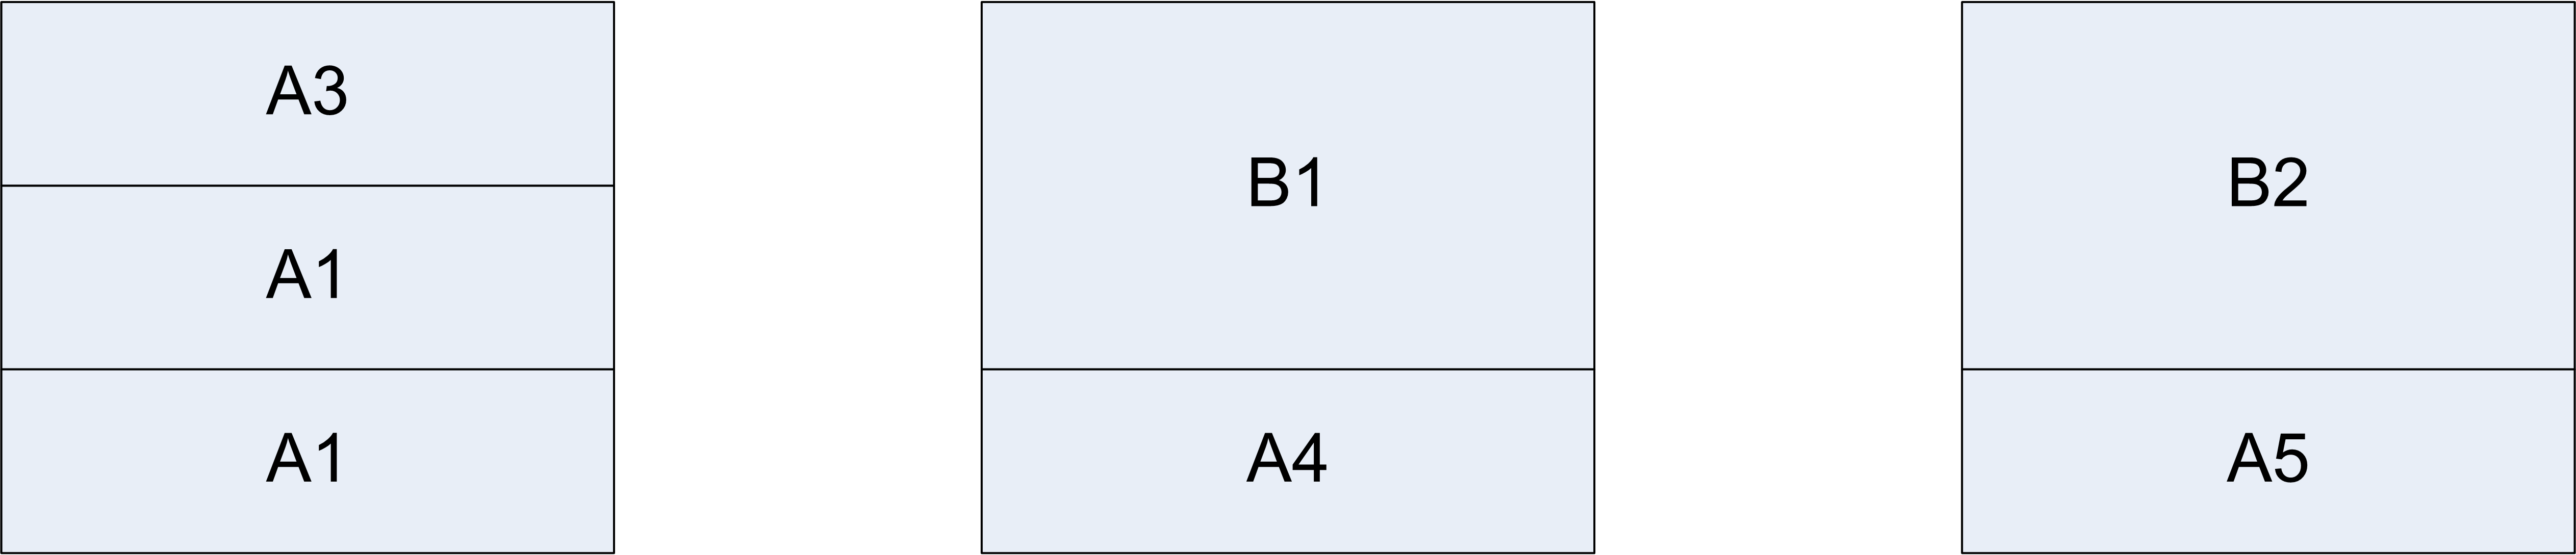
\includegraphics[width=5.5in]{images/ducc-internals/rm-structure-1.png}
      \caption{Unfragmented Layout}
      \label{fig:rm-fragmentation-1}
    \end{figure}

  However, as time proceeds and jobs come and go, it is possible that job A would get
  allocated as in Figure ~\ref{fig:rm-fragmentation-2}.  Now job B can only get 1 process: exactly HALF it's
  ``deserved'' allocation.  It would be necessary to preempt one of job A's processes to make space,
  even though job A is not above its fair-share allocation.

    \begin{figure}[H]
      \centering
      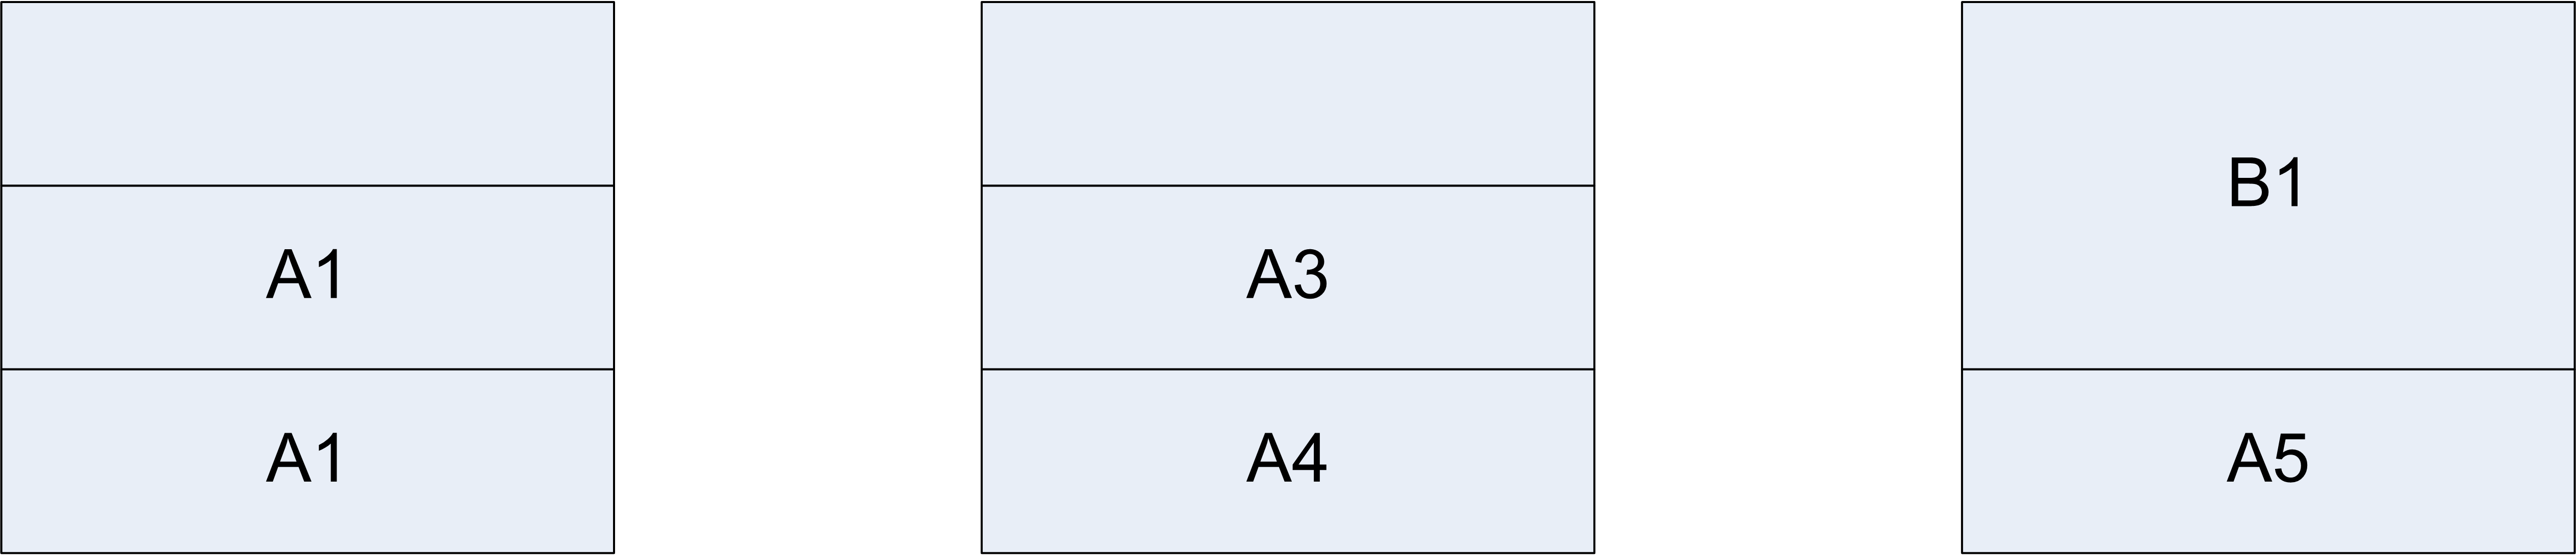
\includegraphics[width=5.5in]{images/ducc-internals/rm-structure-2.png}
      \caption{Fragmented Layout}
      \label{fig:rm-fragmentation-2}
    \end{figure}

  Of course this is a simplistic example.  In general the situation is significantly more complex.

  The goal of {\em defragmentation} is to reconfigure job A as in Figure ~\ref{fig:rm-fragmentation-1} so that
  job B can get its full allocation.

  The general procedure for defragmentation is as follows:

  \paragraph{Detection} This is performed in the method {\em detectFragmentation()}.
  After ``What Of'', all jobs are iterated.  Two numbers  are derived for each job:
  \begin{enumerate}
    \item The number of ``deserved'' shares.  During the ``How Much'' phase, 
      we perform a weighted fair-share assignment of resources. Often a job
      cannot use its full ``fair share'' allotment; for example, it may be a 
      new job and only need two initial processes.  The extra resources are
      apportioned to other jobs which end up with MORE than their proper
      weighted fair-share allotment.

      The ``deserved'' shares is a user's TRUE fair-share allotment, 
      calculated BEFORE bonus shares are allocated to it.  This number is
      calculated during the ``How Much'' phase and stored in each RmJob as
      the {\em pure\_fair\_share}.

    \item The number of allocated shares.  This number is calculated (in {\em RmJob}) as
\begin{verbatim}
   shares_allocated + pending_expansions - pending_preemptions
\end{verbatim}
    \end{enumerate}

    If the number of ``deserved'' shares is greater than the number of allocated
    shares (accounting for expansion and preemption), the job is considered
    ``potentially needy''.

    If there are no ``potentially needy'' jobs, {\em defragmentation} is done and
    we can proceed to broadcast the schedule.

    The second goal of defragmentation is to minimize ``churn'' in the system.  We
    do NOT attempt to achieve a perfect layout.  Instead, there is a threshold
    minimum number of processes we try to guarantee every job.  This number is configured
    in {\em ducc.properties} as the {\em ducc.rm.fragmentation.threshold}.

    A pass is now made over every ``potentially needy'' job.  Every such job with an
    allocation that is greater than the {\em fragmentation threshold} is removed from the
    ``needy'' list.  All remaining jobs are considered ``actually needy''.

    If there are no ``actually needy'' jobs, {\em defragmentation} is done and we can
    proceed to broadcast the schedule.

    Otherwise, the method {\em doFinalEvictions()} is called to try to make space for
    ``actually needy'' jobs.  We perform a ``take from the rich and give to the poor''
    procedure to insure that jobs whose allocation are below both their ``deserved fair share''
    and the ``fragmentation threshold'' are assigned additional resources.

    NOTE: This procedure works for non-preemptable allocations as well.  For non-preemptable
    allocations, the ``deserved'' value is exactly 1 {\em nshare} and any such job
    with no allocations is considered ``actually needy''.

    We iterate all users and add up the total {\em qshares} occupied by all their jobs,
    ordering the users by this value, known as their ``wealth''.

    We iterate the ``actually needy'' jobs.  For each such job we iterate the ``wealthy'' users,
    starting from the ``wealthiest'', inspecting their jobs to see if any of the processes are
    allocated over resources that can be allocated to the needy job.  Note that removal of a share
    must NOT result an an otherwise non-needy job becoming ``needy''.  If so, the user's wealth is
    decremented and one of two things occurs:
    \begin{enumerate}
      \item If the selected process is a ``pending expansion'' that has not been published,
        it is immediately reassigned to the needy job.  (Note that this is an optimization and
        the one exception to the rule that once a allocation is finalized in {\em RmJob}
        it cannot be changed.) If the job is no longer needy it
        is removed from the needy list.
      \item Otherwise, the selected process is preempted and the needy job is placed on
        a global ``needyJobs'' list.  Jobs on this list get priority allocation BEFORE
        any new allocations are made in all subsequent scheduling cycles, until they
        are no longer needy.
    \end{enumerate}
    
    Note the conditions which must be met by a process before it can be donated to a needy job
    (verified in method {\em takeFromTheRich()}):
    \begin{itemize}
      \item The machine containing the share must be of sufficient {\em share order}.
      \item The share must be preemptable.
      \item The machine must be in a compatible nodepool.
      \item If this share is evicted, the owning job must not become ``needy''.
      \item If this share is evicted, it must leave sufficient space on the machine for the new
        share.  i.e, if it is impossible to clear enough space on the machine for the needy job,
        there is no point evicting this share. We iterate all shares on the machine at this point
        and try to evict sufficient shares (which of course must belong to ``wealthy'' users) to
        make space for the needy share.
    \end{itemize}
             
\subsection{NodePool}

    The {\em NodePool} object manages physical nodes, represented in the RM by an
    object called {\em Machine}.  The collections of NodePools form a tree structure
    with each ``nested'' nodepool managed as a ``child'' of its ``parent'' nodepool.
    
    There are many more methods in NodePool than are documented here.  In this section
    we only review the most important, or the most complicated methods.

    The RM supports multiple disjoint NodePools, known as ``top-level'' nodepools.  The collection
    of ``top-level'' nodepools partitions the entire nodespace into independently scheduled
    resource collections.  The motivation is to permit multiple, disparate collections of nodes to
    be managed under a single DUCC system (rather than run multiple independent DUCC systems).

    Most of the NodePool algorithms are recursive.  Both the {\em Scheduler} and
    {\em NodePoolScheduler} object generally interact with the top NodePool of each
    tree, which coordinates, through recursion, the direction of requests to the 
    correct, possibly nested target NodePool.

    For example, to count the machines in a nodepool, one generally wants the count of
    machines in the pool PLUS the machines in its children:
\begin{verbatim}
    /**
     * How many do I have, including recusring down the children?
     */
    int countMachines()
    {
        int count = allMachines.size();
        for ( NodePool np : children.values() ) {
            count += np.countMachines();
        }
        return count;
    }
\end{verbatim}

    In the cases where recursion is to be inhibited, most of the methods are modified
    with the name ``Local'':
\begin{verbatim}
    /**
     * Non-recursive machine count.
     */
    int countLocalMachines()
    {
        return allMachines.size();
    }
\end{verbatim}

    Most of the methods in {\em NodePool} are short and easily understood, like the two above. There
    are a few subtleties in NodePool which will be expanded upon below.

\subsubsection{NodePool Reset}
    All scheduling phases must be aware of what physical resources are available, which are in use, and
    which are available for scheduling.  As we proceed with scheduling we need to maintain scratch-space
    that represents the current ``potential'' schedule, but without perturbing the existing allocations.
    
    The NodePool provides exactly this scratch space.  Before the two main scheduling phases, ``How
    Much'' and ``What Of'', the NodePool is instructed to reset().  The NodePool (and recursively,
    the entire set of nested NodePools), drops all of its structures other than the most basic Machine
    structures and then rebuilds them from the machine structures..  The scheduling phases then create
    ``trial'' schedules, resetting the NodePool as often as necessary.

    This also has the side-effect that errors do not tend to accumulate in the system; we essentially
    reboot the schedule on every pass.

    Finalizing the schedule is done in the Machine objects, with some help from the RmJob and
    Share objects.  

    (NOTE: as an optimization, RM does NOT generally rebuild Machine and RmJob from scratch on each
    Orchestrator publication.  They ARE rebuilt whenever RM starts, and during dynamic RM Reconfiguration).

    The next section, {\em Virtual Machines} provides a concrete example of the use of NodePool for
    scratch space during scheduling.

\subsubsection{Virtual Machines}
    Probably the most important part of the scheduler is encapsulated in the NodePool method,
    {\em rearrangeVirtual}.  This method treats the collection of all ``real'' machines as
    a collection of ``virtual'' machines which is the resource set that is scheduled against.

    In the RM's view, a ``virtual machine'' is any PROPER subset of a ``real machine''.  (Recall
    the mathematical definition of a PROPER subset is any subset of some set that is not equal
    to that set.). 

    As soon as an allocation of a single {\em nshare} is made against a machine, that machine's
    capacity for further allocations is diminished until the allocation is released by the Orchestrator.  For example, an
    order-3 allocation against an ``real'' order-5 machine results in the diminution of the order-5 machine
    to a ``virtual'' order-2 machine.  To put it differently, making a 3-quantum allocation against a 5-quantum
    ``real machine'' results in a 2-quantum ``virtual machine''.
    

    To understand what {\em rearrangeVirtual()} does it is important to understand three tables.
    These three tables are indexed by {\em share order} and are the key structures for both ``How
    Much'' and ``What Of''.  These tables are:
    \begin{description}
      \item[nMachinesByOrder] This table contains the number of full, free ``real machines'' with no allocations,
        indexed by {\em share order} 1, 2, ... {\em maxorder}.
      \item[vMachinesByOrder] This table contains the number of ``virtual machines'' indexed by {\em share order.}
      \item[nSharesByOrder]  This table contains the number of {\em nshares} of every order which can be
        currently allocated.
    \end{description}
    
    There is no overlap between ``nMachinesByOrder'' and ``vMachinesByOrder''. Therefore, the number
    of schedulable ``machines'' of any kind for some specific order {\em O} is
\begin{verbatim}
    nMachinesByOrder[O] + vMachinesByOrder[O]
\end{verbatim}

\paragraph{nSharesByOrder} is derived from the two machine tables and the meaning of its values
    is subtly different.  The numbers in the machine tables are independent of each other.  For example, if
    there is a single order-5 ``real machine'', this does NOT imply that there is also an order-3
    ``virtual machine'' and an order-2 ``virtual machine''.  This breakdown can only happen after
    allocation.

    {\em nSharesByOrder} however, gives the number of {\em nshares} of an order that might be
    allocated from any possible machine, real or virtual, allowing that a larger share may need to
    be split.  Each value in the table is dependent on the values of higher order in the table.  For
    example, if there is 1 order-5 ``real machine'', nSharesByOrder will indicate there is 1
    order-5 share available, or 1 order-4 share, or 1 order-3 share, or 2 order-2 shares, or 5
    order-1 shares.  Here is an example of what these tables might look like at some point during scheduling:
\begin{verbatim}
    Order                     1  2 3  4
    -------------------  ----------------
    nMachinesByOrder[];  [ 0  2  0 1  4 ] - physical machines
    vMachinesByOrder[];  [ 0  1  2 0  0 ] - virtual machines
    nSharesByOrder[]  ;  [ 0 26 11 5  4 ] - collective N Shares for each order
\end{verbatim}
    
\subsubsection{rearrangeVirtual(Machine M, order O)}
    We can now explain this method.  This is called when we wish to allocate a single
    {\em nshare} of order {\em O} from machine {\em M}.  The accounting works as follows:
    if the machine has no allocations, decrement {\em nMachinesByOrder[O]} by one; else
    decrement {\em vMachinesByOrder[O]} by one.  If the allocation would cause the 
    free space to be split, calculate the order of the free space after allocation and 
    increment the correct value in {\em vMachinesByOrder} like this:

    \paragraph{First Step}: Update the two machine tables.
\begin{verbatim}
    int v_order = M.getVirtualShareOrder();    // How much free space in the machine?
    int r_order = M.getShareOrder();           // How much total space in the machine?

    if ( v_order == r_order ) {                // Free == total?
        nMachinesByOrder[r_order]--;           // Yes, full machine allocation
    } else {
        vMachinesByOrder[v_order]--;           // No, virt machine allocation
    }

    v_order -= O;                              // Does it cause a split?
    if ( v_order > 0 ) {                       // Yes
        vMachinesByOrder[v_order]++;           // Add a "new", smaller virt machine
    }
\end{verbatim}
    There are, of course, additional details, which can be seen by inspecting the
    full source listing.

    \paragraph{Second Step} Update the share table.  We initialize the table with the total of real
    and virtual machines by order.  Then in a double iteration, look ``forward'' to count the number
    of shares that might be acquired from higher order allocations by splitting the space.  The full
    method is included here for the curious.  Everyone else can simply trust that it is correct.
\begin{verbatim}
    protected void calcNSharesByOrder()
    {
        int len = nMachinesByOrder.length;

        // init nSharesByorder to the sum of 'n and 'v MachinesByOrder
        System.arraycopy(nMachinesByOrder, 0, nSharesByOrder, 0, len);
        for ( int i = 0; i < getMaxOrder() + 1; i++ ) {
            nSharesByOrder[i] += vMachinesByOrder[i];
        }

        for ( int o = 1; o < len; o++ ) {                     // counting by share order
            for ( int p = o+1; p < len; p++ ) {
                if ( nSharesByOrder[p] != 0 ) {
                    nSharesByOrder[o] += (p / o) * nSharesByOrder[p];
                }
            }
        }
    }
\end{verbatim}
    
\subsubsection{connectShare(Share s, Machine m, IRmJob j, int order)}
    This helper method is responsible for updating all the records in order to
    allocate a specific share on a specific machine for a specific job.  Its
    action is irreversible: once this method is called, the share is irrevocably
    assigned to the given job on the given machine (except sometimes, during
    defragmentation, as described above).

    {\em rearrangeVirtual()} is called at the end to update the internal ``counts''.

\subsubsection{compatibleNodepool(Policy p,  ResourceClass rc)}
    This method determines if the current nodepool is compatible with the indicated
    scheduling policy and resource class.  If the policy is FAIR\_SHARE, recursion
    through the child nodes is performed.

\subsubsection{nodeArrives}
    This straightforward method adds a node to the list of schedulable nodes.  It updates the
    database, deals with unresponsive nodes becoming responsive again, and does
    simple bookeeping.

\section{RmJob}

    The RmJob is mostly an accounting object.  While its implementation has many details,
    there are two important methods: {\em calcJobCaps()} and {\em shrinkBy(int count)}, both
    of which were briefly mentioned above.

\subsection{calcJobCaps()}
    If the {\em rearrangeVirtual()} code described above has a rival for ``most important method'',
    it would be the RmJob's {\em calcJobCaps()}.  This method is called many times throughout
    scheduling and is required to return {\em exactly} the number of shares the job could make
    use of at the current moment, if there were unbounded resources.

    Note that this is the method to modify if you wish to change the rate of expansion or
    contraction of a job.

    Because it is called so often, the scheduler iterates all jobs at the start of each 
    scheduling cycle and calls {\em initJobCap()} to calculate the cap based on current job
    state.  This caches the actual cap, which is returned in subsequent calls to
    {\em calcJobCaps()}.

    The design point is this:  Estimate the cap as the largest value that is meaningful.  Then
    whittle it down to the minimum by applying the architected constraints such as
    the ``initialization cap'' and prediction of when we expect the job to complete.  We want
    everything we can get but no more than we can use.

    This code can be tricky to understand so we'll present it here.  The returned ``actual\_cap'' is
    the value used by NodePoolScheduler's ``How Much'' phase for all {\em entities} to determine share allocations.

    The following steps are taken by {\em initJobCap()}:
    \begin{enumerate}
      \item If the job is unschedulable (refused), set cap to 0 and return. (No shares will be allocated.)
      \item If the job is completed but not yet deallocated, set the cap to the total shares
        it already has allocated and return. (No additional shares will be allocated.)
        \item Set the tentative cap to the number of remaining {\em work items}  divided by the declared
          threads per processes.  This is the upper bound on the cap:
\begin{verbatim}
     c = (n_remaining_questions / nthreads}
\end{verbatim}

        \item Adjust the tentative cap to the maximum of ``c'' and the number of shares already
          allocated.  This accounts for jobs ``winding down'' when work items start to vacate
          processes so we have more processes than are needed for the remaining work but we 
          want to insure that ``How Much'' does not cause premature shrinkage.
\begin{verbatim}
        int currentResources = countNShares();
        c = Math.max(c, currentResources); 
\end{verbatim}

        \item Adjust the tentative cap to the minimum of ``c'' and the declared {\em process\_deployments\_max}.
          Call this the ``base cap''.  It is the job cap before accounting for prediction and is
          used if we cannot find a better estimate.
\begin{verbatim}
        int base_cap = Math.min(getMaxShares(), c);
\end{verbatim}
          
        \item Predict the number of shares this job could use on an unbounded system,
          based on the average initialization time of its processes and the rate of completion
          of the work items so far.  Call this the ``projected\_cap''.
\begin{verbatim}
        int projected_cap = getProjectedCap();      
        if ( projected_cap == 0 ) {                   // we know nothing, this is best guess
        	projected_cap = base_cap;
        }
\end{verbatim}

        \item All else being equal, the potential cap for the job is now the max of the actual
          resources we have allocated, and the projected cap.  It is the largest number of
          resources we believe the job can ever use.
\begin{verbatim}
        potential_cap = Math.max(projected_cap, currentResources);
\end{verbatim}

            \item If we're still initializing, and we have configured {\em ducc.rm.initialization.cap}
              in {\em ducc.properties}, revise the cap down and return the {\em actual\_cap}.
\begin{verbatim}
        actual_cap = Math.min(potential_cap, (resource_class.getInitializationCap()));
\end{verbatim}

            \item If we're still initializing and we do NOT have an initiation cap configured,
              set the {\em actual\_cap} to the {\em potential\_cap} and return.
\begin{verbatim}
        actual_cap = potential_cap
\end{verbatim}
              
            \item If we've completed at least one initialization, and we have configured
              {\em ducc.rm.expand.by.doubling}, return the smaller of the {\em potential\_cap}
              and TWICE the currently allocated resources:
\begin{verbatim}
       actual_cap = Math.min(potential_cap, currentResources * 2);
\end{verbatim}

            \item If we've completed at least one initialization, and we do NOT use
              expand-by-doubling, return the {\em potential\_cap}
\begin{verbatim}
       actual_cap = potential_cap
\end{verbatim}

              \item There is one last corner case.  It is possible the job has
                shrunk to 0 resources (pushed out by fair-share for example). If
                this has happened we have to restart the doubling, and we need to
                ask for at least the initialization cap.  But we don't want to go
                over the ``base\_cap'' which has accounted for the fact the job might
                be running down and we can't use the full initialization cap.
\begin{verbatim}
      if ( currentResources == 0 ) {
         actual_cap = Math.max(1, resource_class.getInitializationCap()); 
         actual_cap = Math.min(base_cap, actual_cap);                     
       }
\end{verbatim}


        \end{enumerate}
    
\subsection{shrinkBy(int count)}
    This is a rather trivial method, used to implement ``shrink by investment''.  Originally
    this was a much more involved processes, which gradually became refined to its current
    incarnation.

    All this method does is sort the RmJob shares as described in the interlude above, ``Preemptions'',
    and deletes the indicated number of shares from the front of the sorted list.

    The original {\em shrinkByInvestment()} code has been left in place for reference.

\section{Supporting Classes}
   There are a number of supporting classes mostly used for bookkeeping, mentioned here for completeness.

\subsection{Machine}
This represents a Node.  A Machine object is created whenever a Node's state arrives.  The Machine
is entered into an appropriate nodepool.  Machine objects are NEVER destroyed (except during dynamic
reconfiguration) as it is usually expected that an unresponsive machine will become responsive
again.  This significantly reduces the complexity of bookkeeping.

\subsubsection{Blacklists and Whitelists}
The Machine maintains a list of {\em Share}s allocated to it.  It is possible, after changing the
{\em ducc.classes} configuration and starting RM, that it is no longer legal for these shares to be
allocated on this machine, or perhaps to be allocated at all.  For example the machine may have been
moved to a different class than the class of the work allocated on it, or the class may be been
deleted entirely.

   If this happens the shares are essentially in ``limbo''.  They cannot (in general) be associated
   with any resource class and therefore cannot participate in allocations (recall, allocations are
   done by resource class).  The space must nonetheless be accounted for to avoid double-booking the nodes.

   To cope with this the RM considers both the {\em Shares}, and the {\em Machine} they reside on
   to be ``blacklisted''.  When a machine is ``blacklisted'',
   \begin{itemize}
     \item All work that can be evicted from it is evicted.  This include any kind of UIMA-AS
       job (including jobs submitted to non-preemptable classes),  and Services.
     \item No additional allocations can be made to the machine until ALL blacklisted work
       has been confirmed by the Orchestrator to have left the system.
   \end{itemize}
   
    Once all blacklisted work on a machine has left the system, the machine is ``white-listed'' and
    allocations on it are resumed.

\subsubsection{Database and Persistence}
   When any machine arrives in the system, a new record is entered in the database containing its
   essential data.

   All state subsequent changes for the machine are entered into the database, including the number
   of missed consecutive Agent heartbeats.

   When a share is assigned to a machine, or leaves a machine, it is the responsibility of the Machine object to
   record the share and its details in the database.

\subsection{Share}
    The Share object represents one full allocation.  Internally it is an {\em nshare} and thus
    has share order, where the {\em share order} is the number of {\em qshares} it represents.  A
    share is logically exposed outside of RM as a Process.

    The Share's main purpose is bookkeeping; a place to store investment, initialization time and
    to represent the space occupied by a resource allocation.

\subsection{ResourceClass}

    The ResourceClass represents the {\em class} concept as configured in {\em ducc.classes}.  It
    holds the configured class rules (expand\_by\_doubling, initialization\_cap, etc).

    It's primary purpose is bookkeeping; a place to organize jobs by class, jobs by user by class,
    to maintain the set of users authorized for the class, etc.  It also tracks non-preemptable
    share {\em allotment}.

    The {\em ResourceClass} is a schedulable {\em IEntity}, as described above in the description
    of the FAIR\_SHARE algorithm.

\subsection{User}

    The User represents a single user. Its primary purpose is bookkeeping; a place to organize
    jobs owned by the user.

    The User is a schedulable {\em IEntity}, as described above in the description of the 
    FAIR\_SHARE algorithm.

\subsection{JobManagerUpdate}

    This is a ``transfer object'' used to transfer the current schedule to the publication
    mechanism and ultimately to the Orchesrator.  It consist of maps of all shares, organized
    by shares ``expanded'', and ``shrunken'' (preempted).  The RM's publication mechanism
    translates this into the appropriate format which then gets published to the Orchestrator.
    


\chapter{Service Manager}
% 
% Licensed to the Apache Software Foundation (ASF) under one
% or more contributor license agreements.  See the NOTICE file
% distributed with this work for additional information
% regarding copyright ownership.  The ASF licenses this file
% to you under the Apache License, Version 2.0 (the
% "License"); you may not use this file except in compliance
% with the License.  You may obtain a copy of the License at
% 
%   http://www.apache.org/licenses/LICENSE-2.0
% 
% Unless required by applicable law or agreed to in writing,
% software distributed under the License is distributed on an
% "AS IS" BASIS, WITHOUT WARRANTIES OR CONDITIONS OF ANY
% KIND, either express or implied.  See the License for the
% specific language governing permissions and limitations
% under the License.
% 

% \section{DUCC Service Manager}
    This section describes the architecture and internal structure of the
    DUCC Service Manager, referred to as the ``SM''.

\section{Introduction}
    The SM function is to insure that any services needed by
    DUCC jobs are running and functional at the time they are needed by
    jobs.  Previous to the incarnation of the SM it was necessary for
    users to manually invoke the processes implementing their services.  If
    these processes were to crash, jobs dependent on them would stop until
    some human was able to restart the service.  If the operating system,
    or batch system supporting the jobs (DUCC, in our case) was to
    be restarted, users would again have to manually start the services.

    By ``registering'' a service with the SM, a user can trust DUCC to
    keep the service alive and functional across all manner of faults and
    system restarts.  As well, the SM has a mechanism for ``testing'' a
    service to determine if it is operational, and to inform the DUCC
    Web Server when it is not.  

    If a user submits a job that declares a dependency on a service, the SM
    is able to start the service as needed, and is able to stop the service
    when no longer needed, freeing resources.

    In essence, the SM can be thought of as a ``proxy user'' dedicated
    to insuring that services are always available when needed.

\section{Architectural Overview}

    Figure ~\ref{fig:sm-structure} below shows the high-level object,
    threading, and process structure of SM and should be referenced
    while reading this document.
    
    The SM can be pictured as being composed of four major parts:
    \begin{enumerate}
      \item Initialization and interaction with external components.
        External components include user requests and  other DUCC components such as
        the Orchestrator.
      \item A ``Service Instance'' manager.  This part resolves
        dependencies on services, starts and stops service instances
        according to the needs of jobs and the policies declared in
        the service registries, and handles the service instance
        lifetimes.
      \item A ``Service Health'' manager.  This part continually
        ``tests'' services to determine whether they are 
        functional.  This is referred to as the ``pinger'' and the
        test is known as a ``ping''.
      \item A ``CLI Handler'' which reacts to requests from users.
    \end{enumerate}

    \begin{figure}[H]
      \centering
      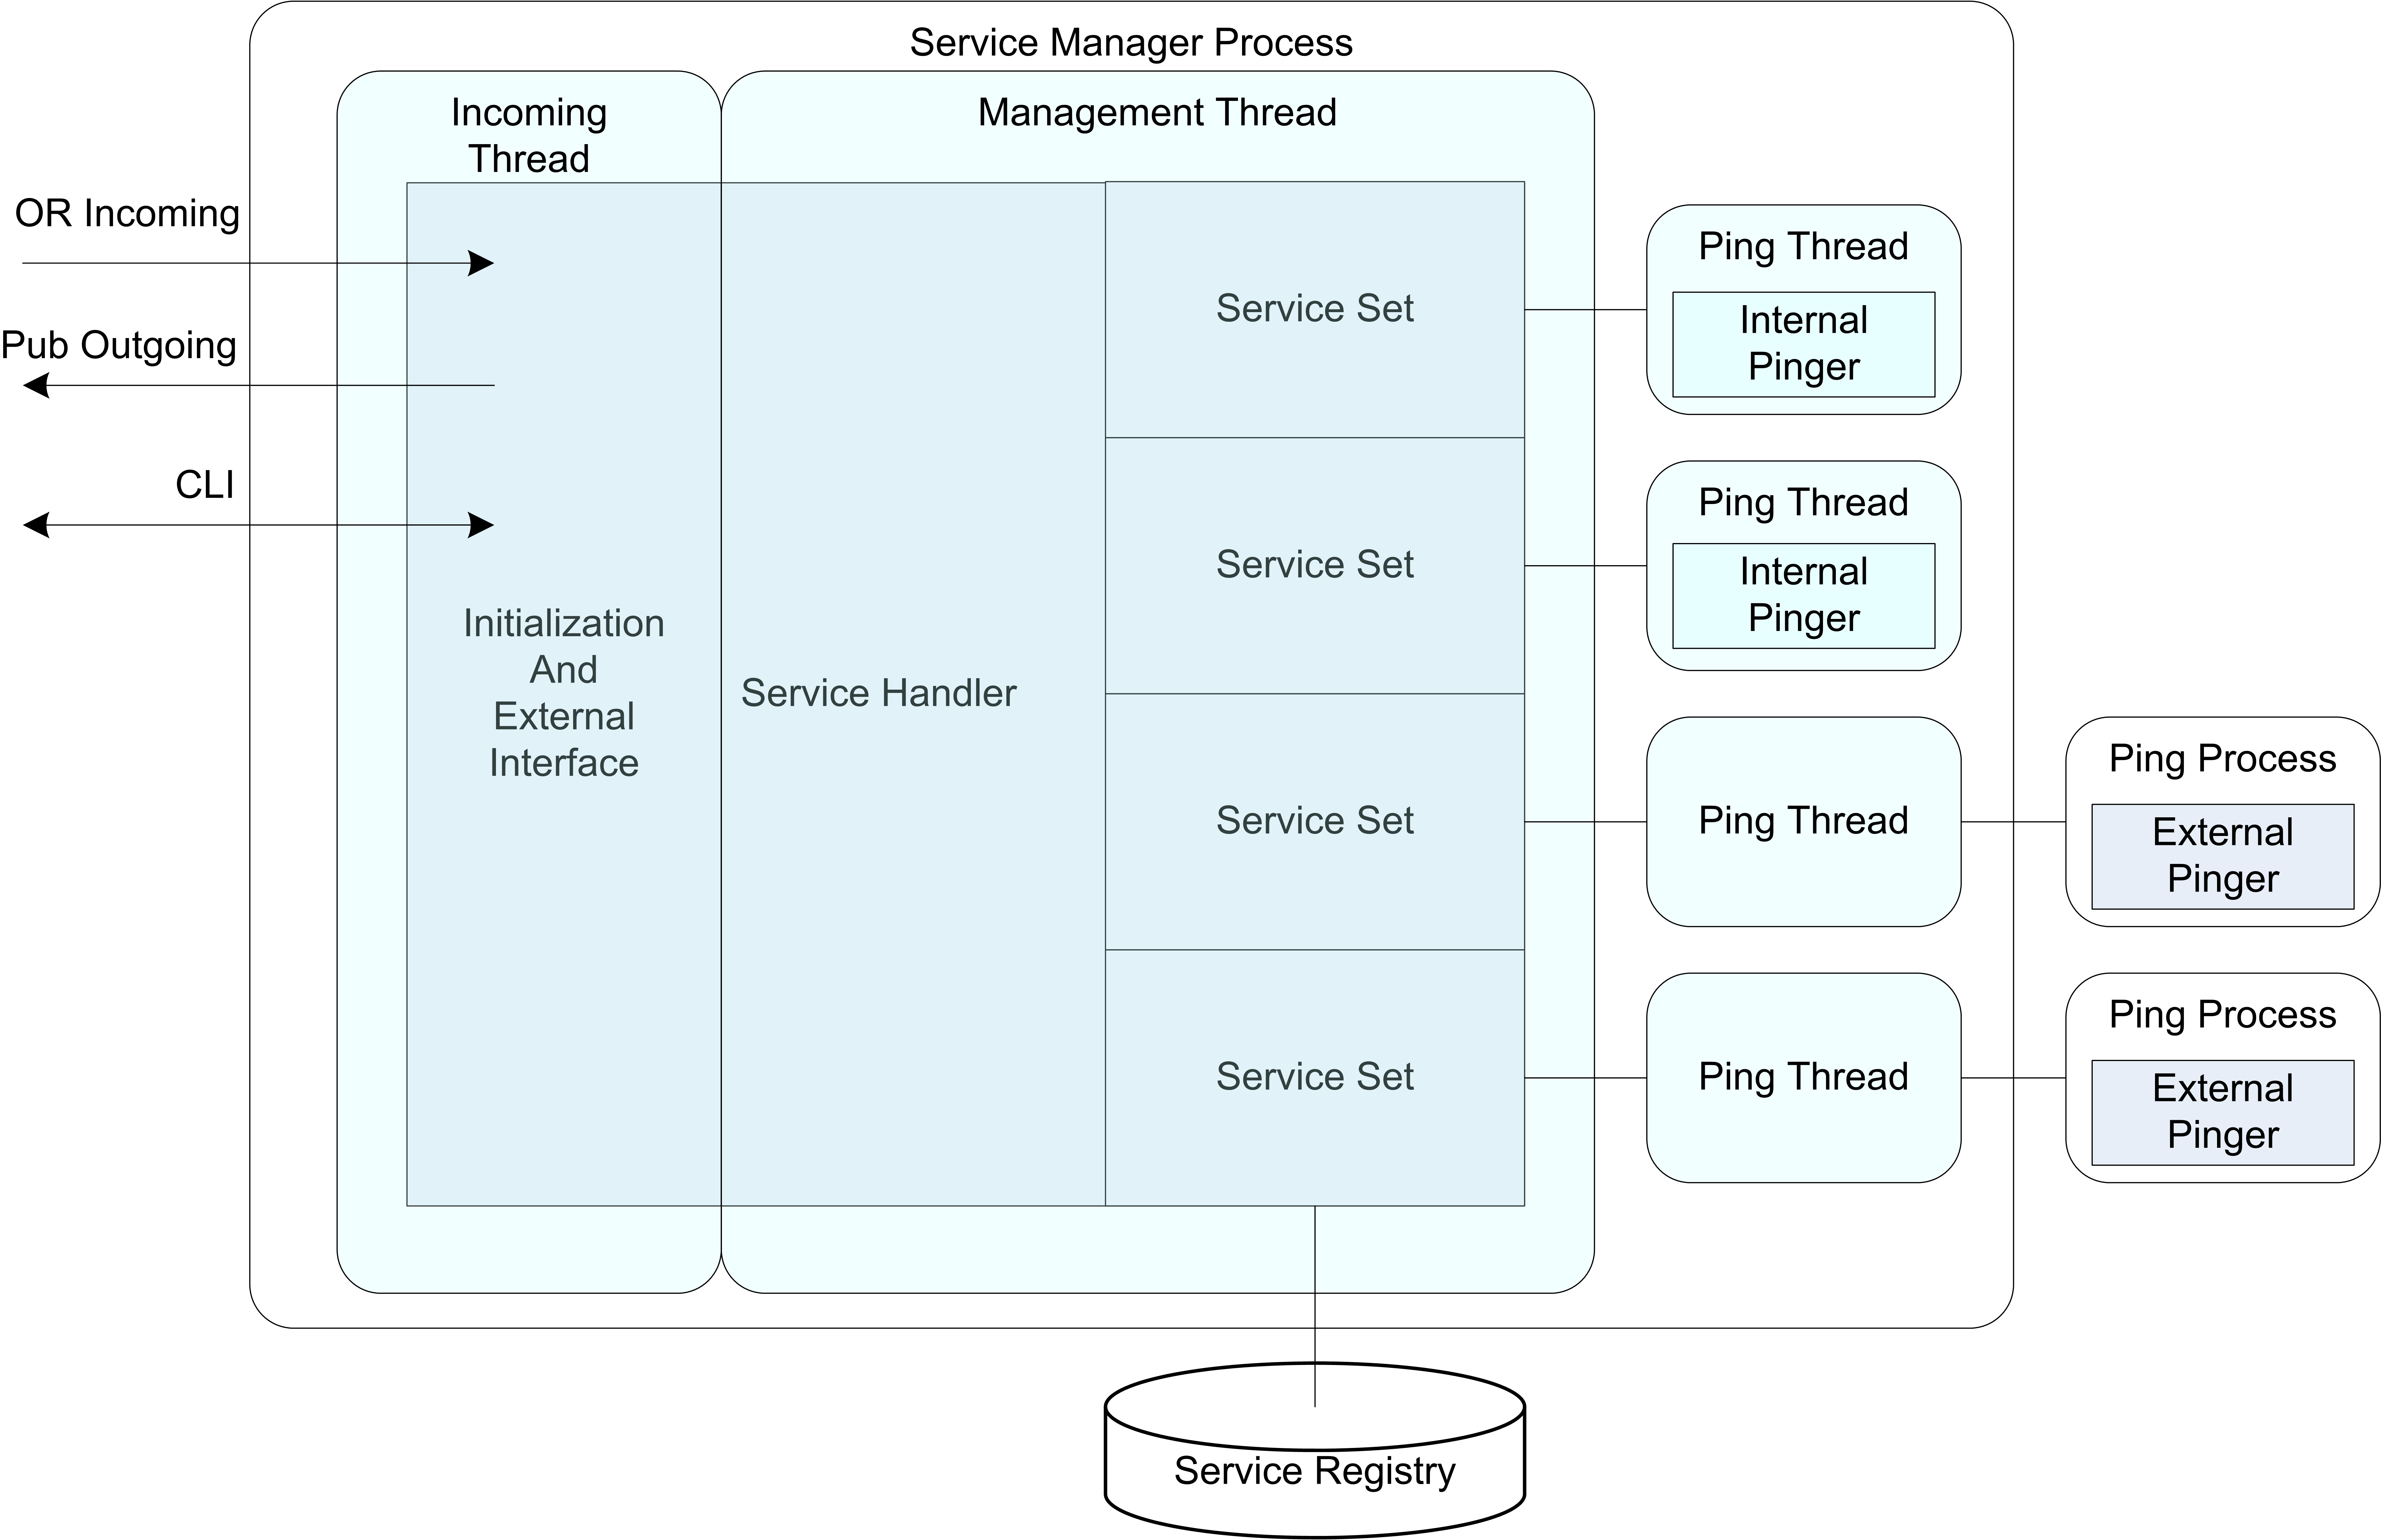
\includegraphics[width=5.5in]{images/ducc-internals/sm-structure.png}
      \caption{Service Manager Structure}
      \label{fig:sm-structure}
    \end{figure}

   The terminology around Services can be confusing.  We review the ideas here.

   There are three ``countable'' entities involved in services.  
   \begin{description}
     \item[Service Registration] When a service is ``registered'' the Service Manager assigns
       a new, unique {\em Registration ID} to the registration.  This ID is associated with, and
       remains with, the service throughout its lifetime and beyond when it is archived.

     \item[Service Instance] When the Service Manager starts a service it issues a series of
       ``submit'' orders to the Orchestrator, one for each {\em Service Instance}.  All these 
       instances are associated with the {\em Service Registration}.  The orchestrator assigns
       a unique ID to each service instance, which is also permanently associated with that entity.
       
       This is analogous to a {\em job}, but with a single allocation.  The SM organizes
       multiple {\em Service Instances} under a single {\em Service Registration}.
       
     \item[Share Id] When an instance is submitted to the Orchestrator, the Orchestrator
       ``submits'' a request to the Resource Manager to find resources.  Each instance is
       treated independently by the RM.  When a resource is found for the instance, the RM
       assigns a {\em Share ID} to the allocation. 
       
       This is analagous to a {\em job's} process or ``PE''.
    \end{description}

    The {\em Service Registration} ID appears on the Services' page of the webserver.  The {\em
      Service Instance} ID and the {\em Share Id} appear in the ID column of the service details in
    the DUCC webserver.  For example, this ID: {\tt 289661.34094} indicates {\em Service Instance}
    ID {\tt 289661} and {\em Share Id} {\tt 34094}.

\section{Initialization and Interaction with DUCC}
   The component responsible for initialization and external interaction is
   implemented in the source file {\em ServiceManagerComponent.java}.  This
   straightforward bit of code performs the following functions, details of which
   are easy to understand by reading the source code itself.  

   \begin{description}
     \item[Initialization] This consists of the methods init() and
       start(). The DUCC framework instantiates ServiceManagerCompoent and calls
       its start() method.  This initializes various structures from
       {\em ducc.properties}, initializes the database connection, and
       initializes the two main threads:
       \begin{enumerate}
         \item The SM proper, {\em ServiceManagerComponent}, which
           fires its {\em run()} method which in turn calls {\em init()}.
           \item The Service Instance manager, implemented in {\em ServiceHandler.java}.
       \end{enumerate}
       The {\em init} method reads all registrations from its state repository and
       passes them to {\em register()} (using the same code path as the {\em register} CLI),
       to establish them in a memory map and possibly initialize them.


       \item[Interaction With DUCC] There are three primary interactions to be aware of:
         \begin{enumerate}
           \item Incoming Orchestrator publications.  This arrives on an external
             communication thread  and passed to
             the method {\em orchestratorStateArrives} which, if it accepts the
             publication, saves the incoming publication and issues a {\em notify()} to 
             the main {\em ServiceManagerComponent} thread to allow processing of the state.  

             The method {\em processIncoming} is then called which does standard DUCC
             state-differencing and passes updates to the {\em Instance Management} code
             in {\em ServiceHandler}.

           \item CLI requests.  These are passed via the usual DUCC event handlers to specific
             second-level handlers, one for each type of CLI request (e.g. {\em register()}).  Each of these
             second-level handlers is responsible for these actions:
             \begin{description}
               \item[User validation.]  Insure the caller of the CLI is {\em authenticated}, i.e.
                 is the user he claims to be.
               \item[Ducc is running.]  The DUCC Orchestrator must be actively publishing state
                 before SM is allowed to interact with users.                 
             \end{description}
             
             If these simple tests are passed, the request is passed to the Instance Management
             code in {\em ServiceHandler} to check for authorization (i.e. is this user allowed
             to perform this action against this service).  

           \item Outgoing state publications.  Outgoing state is a simple map, one entry per
             job (a ``job'' for SM is any unit of work in the system: UIMA-AS job, Service instance,
             Reservation, AP).  The entry contains the state of the job relative to any
             services it depends on, which is interpreted by the Orchestrator and Web Server.

         \end{enumerate}

         Note that Orchestrator publications and CLI requests may be ignored under these two conditions:       
         \begin{enumerate}
         \item SM initialization is not complete.  Completion is flagged as the last
           action of {\em init()}.
         \item RM has not yet assigned the JD node.  The incoming OR publication includes a flag to
           indicate whether the JD node is assigned.  We have to wait here because we do not want
           the SM to process work or initialize any services until it is confirmed that the system
           is fully initialized.  Note that this minimizes the occurrence of errors and simplifies
           error management because you can all errors occurred in a fully initialized environment.
         \end{enumerate}
         
     \end{description}
   

\section{Service Instance Management: ServiceHandler and ServiceSet}
    After the differencing engine has determined the various work events that have
    occurred, the Service Instance Management code examines each event
    and acts upon it.  

\subsection{Operational Overview}
    The code described below runs in a thread separate from the main thread
    described in the previous section.  Incoming events are placed on lists
    segregated by function (a list for new Jobs, a list for updated Jobs, etc).  As soon
    as all incoming events are placed on these lists the {\em Service Instance Management}
    thread is {\em notified}.  The {\em Service Instance Management} thread sets a lock,
    drains the lists into internal structures, and releases the lock.  This segregates the
    the actions of the {\em ServiceManagerComponent} from {\em Service Instance Management}.

    As incoming events are acted upon, a summary of the service state for all
    incoming work is built up.  After all events are processed, the {\em ServiceManagerComponent} 
    (previous section) is notified and the state publication is sent to the Orchestrator.

    There are two primary components involved in {\em Service Instance Management:}
    \begin{description}
      \item[ServiceHandler.java] This is a singleton object which runs in its own 
        thread sepparate from the {\em ServiceManagerComponent}.  It fields the
        updates from the Orchestrator and CLI, resolves Service dependencies, and signals
        the {\em ServiceSet} for each affected service so appropriate action can be taken.
        It maintains all the records of registered services and service-dependent jobs
        in an inner class {\em ServiceStateHandler}.
      \item[ServiceSet.java] There is one {\em ServiceSet} for every registered service.  It is
        instantiated on receipt of a registration and destroyed only when a service is unregistered.
        It is responsible for submitting service instances to the Orchestrator, reacting to state
        changes of the Service Instances, enforcing management policies ({\em reference start}, {\em
          autostart}, {\em manual start}), and fielding the data from the service Pinger.
    \end{description}
      
\subsection{ServiceHandler.java}
    The work-related events, fielded by {\em ServiceHandler}, are described below.
    These events can be placed into two broad categories:
    \begin{enumerate}
      \item Events relating to work that requires services, usually UIMA-AS jobs
      \item Events relating to service instances for registered services.  
    \end{enumerate}
    
    Within each category are three types of interesting events.
    \begin{enumerate}
      \item A new job or service instance has entered the system.  This is essentially a REQUEST
        from the Orchestrator, asking if all necessary services are available.  No work
        has been started in the system, and will not be until SM responds ``services available''
        to the request.

        NOTE that the Orchestrator has a ``fast-path'' for work that has no service dependencies, in
        that it does not wait for the SM to respond regarding such work.  SM does in fact respond,
        but after the fact, and the response is not used.

      \item An existing job or service instance has changed state.  This is work that the 
        Orchestrator has started: there are physical processes either started, or in the act
        of starting and their states may be evolving.

      \item An existing job or service instance has terminated.
    \end{enumerate}
    
    While technically any type of DUCC work can be dependent on a service, by far the most common
    is UIMA-AS Jobs and Service instances.  The SM must treat work which IS a Service Instance
    a little differently from all other work (because all work is potentially depdenent on the
    state of Service Instances). Below we will use the term ``Job'' to refer to any
    kind of work that is not a service instance.

    NOTE: for simplicity, the descriptions in this section use the term ``services available'' to refer
    to the single state {\em Available} which indicates a service is running and is successfully
    pinging, and  ``services unavailable'' to refer to all other states.  The complete set of
    states is encoded in the class
\begin{verbatim}
org.apache.uima.ducc.transport.event.sm.IService.java
\end{verbatim}
    in the enum {\tt ServiceState} as shown below.
\begin{verbatim}
    public enum ServiceState 
    {
      Pending,        // Work is waiting on at least one service to start
      Waiting,        // A job is waiting on at least one service to ping
      Starting,       // Instance is started, but not yet to Initializing
      Initializing,   // A job is waiting on at least one service to initialize
      Available,      // All services for this job are active and pinging, or else
                      //     no services are needed for the job
      NotAvailable,   // SM to OR only: reference to a non-existent service 
      Stopped,        // The service is not started
      Stopping,       // Service is told to stop but it takes a while
      Undefined,      // Catch-all, means basically "who cares"
      ;
    }
\end{verbatim}

    \paragraph{Service Events}. Service events are {\em processed in the order shown
    below.} The order is important because overall service state is advancing through the
    first three events.
    
    \begin{description}
      \item[A new Service Instance has arrived.]  The associated {\em ServiceSet}
        is found and signalled.  If the associated {\em ServiceSet} cannot be found this
        is considered a ``rogue'' service instance and is ignored.  This occurs if
        the incoming process cannot be matched with a registered service; for example, if
        the {\em DuccServiceSubmit} CLI is called outside of SM.  Usually this is an
        error condition but is not considered fatal by SM.

        If this service is dependent on other services, the {\em ServiceSet}s for those
        other services are fetched and signalled, which may in turn cause additional
        service instances to be submitted.  If all of these other services are Running,
        the new service is marked ``services available'' and the Orchestrator will 
        physically start the new instance.  Otherwise it is marked ``services unavailable''
        and will not be allowed to start until it's own service dependencies are running.

        Note how this implements a sort of ``domino'' effect for starting services.  Suppose
        you have two services, A dependent on B, and a job dependent on A,
        with none of these running.  When job A arrives at SM it is marked ``services unavailable'' and
        service A is submitted.  When service A arrives from Orchestrator it is marked ``services unavailable'' and
        service B is submitted.  When service B arrives from Orchestrator it is marked ``services available'' so 
        that Orchestrator may start it.  When it starts, service A is marked ``services available'' and is
        started by Orchestrator.  When service A starts, the job is finally marked ``services available'' and
        is allowed to start.

        As mentioned above, if the services is NOT dependent on other services, the Orchestrator
        will fast-path its start, and SM will mark it ``services available''.
     
      \item[An existing Service Instance has arrived.]  The {\em ServiceSet} is
        fetched and signalled with the state of the incoming instance.  This may cause
        the Service State to be updated, for example from Initializing to Running.  Pingers
        may be started as needed.

        Note that, because this is processed BEFORE jobs are processed, job state may be
        updated from ``services available'' to ``services unavailable'' (or vice-versa).

      \item[A Service Instance has exited.]  Some service instance for some managed
        service has exited for some reason.

        The associated {\em ServiceSet} is found and signalled.  The {\em ServiceSet}
        takes appropriate action, restarting the instance if the exit
        was unexpected, or perhaps simply updating its records if the service is
        being stopped or the number of instances reduced.

      \item[A new job has arrived.]  
        The declared service dependencies are parsed and the {\em ServiceSet}
        object for each such service is signalled.   The {\em ServiceSet} increments the reference count for
        the service and, in the case of {\em reference-started}
        services, starts some number of instances (using the ``hidden'' CLI utility
        {\em DuccServiceSubmit}.

        Based in the current state of the service, the job is flagged with ``services available'' or
        ``services unavailable''.  The job is marked ``services available'' if-and-only-if all
        its declared services are started, in running state, and being successfully {\em tested} (``pinged'').

      \item[An existing job has arrived.]  Work that is not new may need its service state reevaluated.
        The declared service dependencies are parsed and the associated {\em ServiceSet}
        objects are fetched.  An analysis of the combined work states and service
        states is done.  The job is flagged ``services available'' or ``services unavailable''.

        Note that a job's service-state can change from ``services available'' to ``services
        unavailable'' if a service fails for some reason.

      \item[A job has exited.]  A job which might be dependent
        on a service has left the system. 

        The ServiceHandler examines all the declared services for the work.  For each
        dependency, if the service is started, the ServiceSet for the service is 
        signalled.  Each affected {\em ServiceSet} decrements its reference count.  If the
        count goes to zero, and if this is
        a reference-started service, the {\em ServiceSet} stops all instances.
          
    \end{description}
    
\subsection{ServiceSet.java}
{\em ServiceSet} is responsible for the care-and-feeding of the set of objects, threads, and
processes used to manage an individual service.  There is one {\em ServiceSet} instantiated for
every registered service.  {\em ServiceSet} does NOT run in its own thread.  Its methods are always
executed either on the thread of the {\em ServiceHandler} or on a {\em pinger} thread. It is
responsible for maintaining the correct number of running instances, fielding pings, and updating
the state repository (as of DUCC 2.1.0, a database) for a single service.

   The primary functions include:
   \begin{description}
     \item[Enforce Autostart]  If the service is registered for autostart, insure sufficient instances are started
       and start new ones if needed.  This is called at the end of each update cycle from the {\em ServiceHandler}.

     \item[Manage references] Maintain a reference count to reflect all work that is
       referencing the service.  If the service is ``reference started'' this can trigger
       the start of new instances and the shutdown of existing instances.  This count is
       always maintained so if the administrator changes the start-up policy for the service,
       the reference count is already correct and is used.

    \item[Start-up and hot start] On hot-start, the method {\em bootInstances()} is called to
      synchronize each service set with the incoming orchestrator publications, followed by
      bootComplete() to finalize bookkeeping and update the meta state data.

    \item[Field pings] When the Orchestrator state indicates that at least one instance for the
      service is in Running state, the {\em ServiceSet} starts a pinger.  After every ping,
      the pingers call {\em signalReblance()} to respond to the ping and enforce any
      potential state changes as a result of the ping, including starting and stopping 
      specific instances.

    \item[Sequence Instance Startup] The {\em ServiceSet} also sequences instance start-up so that
      in general, there is only a single instance starting at  time.  This is managed in the
      method {\em needNextStart()};

      Instances are sequenced up for several reasons:
      \begin{itemize}
        \item Avoid flooding the system with start requests during boot.
        \item Avoid start/fail loops with faulty services.
      \end{itemize}
      
    \item[Respond to Instance State Change]  The {\em ServiceHandler} invokes the {\em ServiceSet}
      method {\em signalUpdate} on every Orchestrator update.  This method examines the entire
      state of the service and coordinates any actions which may be triggered by state change
      of a service instance.

    \item[State Accumulation]  The state of a service is dependent on the cumulative states of
      all of its instances PLUS the state if its pinger.  The method {\em cumulativeJobState()}
      is responsible for state accumulation.

      The design point is that states are associated with an ordinal.  The larger the ordinal,
      the ``closer to functional'' a service is.  The lower the ordinal, the ``farther from functional''
      the service is.  State accumulation walks the states of all relevant components maintaining
      the {\em maximum} state encountered.  This {\em maximum} is considered to be the state of the
      service overall.  The method {\em translateJobState()} is used to assign the ordinal
      based on the state of the service instances.

    \item[State Management] There is a very simple state machine managed by two methods,
      {\em signal()} and {\em setState()}.  The details can be found by examining these methods.
      The design point is this:  most actions in the SM are considered {\em idempotent}.  Thus,
      regardless of the outcome of state change (or lack of state change), these actions are
      ALWAYS called; for example, ``start the pinger''.  The methods implementing the actions
      are responsible to determine whether the current situation is compatible with the requested
      action.  For example, if the method {\em startPingThread()} is called, that method must
      check to see if the ping thread is already running, and not start a new thread if so.

      This design makes the state machine extremely simple and easy to maintain.

      \item[Lingering Stop] {\em Lingering stop} occurs in a reference-started service when the
        final reference has exited.  It is implemented by a Java TimerTask, {\em LingerTask}.
        If the timer ``pops'', this task stops the service.  If a new reference arrives
        before the timer ``pops'', the task is canceled.

   \end{description}

\subsection{ServiceInstance.java}
    The {\em ServiceInstance} object is a simple helper whose responsibility it is to start
    a new instance.  It spawns a {\em DuccServiceSubmit} process as the user via {\em ducc\_ling} with a pointer to the
    registration properties, and scrapes the output in the response to get the Orchestrator-assigned
    ID.  The ID and any error messages are returned to the calling {\em ServiceSet}.

    This mechanism is used to manage ping-only services as well.  When a ping-only service is started,
    a subclass of ServiceInstance is started.  This {\em PingOnlyServiceInstance} simulates the start
    of an actual instance.  It maintains an internal thread that invokes {\em ServiceSet.signal()} to simulate
    the {\em ServiceHandler}'s regular state updates.  It is essentially a ``service proxy'' for the 
    non-DUCC-handled service that is being pinged, eliminating the need for most special cases in the
    handling of ping-only services.

\section{Service Health Management: Ping support}
    When the {\em ServiceSet} detects that at least one instance has achieved {\em Running} state,
    it calls the method {\em startPingThread()}.

    {\em startPingThread()} starts a thread dedicated to managing the pinger, with the class
    {\em PingDriver} running as its (logical) ``main''.  The {\em PingDriver} reaches back into its
    {\em ServiceSet} for the parameters needed to manage the pinger (Java class, ping interval,
    etc).

    The {\em PingDriver} implements two cases:
    \begin{enumerate}
      \item Internal pingers
      \item External pingers
    \end{enumerate}
    
    In both cases, the {\em PingDriver} object creates an object from {\em Ping.java}, loads
    the object with a {\em Map} of user and DUCC-supplied parameters, and passes the {\em Ping} to
    the ping implementation.  A timer is set and a response is waited for.  

    In both cases the ping mechanism collects ping parameters and passes them to the {\em AServicePing}
    object which was extended to create the pinger.  The ping mechanism then calls various
    methods on {\em AServicePing} to extract its state, constructs a {\em Pong} object, and uses
    this to communicate with the SM by invoking {\em ServiceSet.signalRebalance()}.  The details
    of how this occurs is different for internal and external pingers in the {\em PingDriver}.
    
    \subsection{Internal Pingers}

    If the pinger is registered as an ``Internal'' pinger, a Java ClassLoader is invoked to load
    the pinger's registered class. A timer loop is established to invoke the pinger.  On
    each invocation, the {\em PingDriver} directly invokes the methods on {\em AServicePing} 
    required to invoke the pinger and retrieve its state.  A {\em Pong} object is created
    from the state and passed to common code in the method {\em handleResponse()}.

    \subsection{External Pingers}

    If the pinger is registered as an ``External'' pinger, a ServerSocket is started and its listen
    port acquired. An instance of the class {\em ServicePingMain} is spawned under the identity of
    the owning userid of the service via {\em ducc\_ling}, passing the listen port and appropriate
    arguments needed to start the user's pinger. The stdout and stderr of the resultant process is
    captured and written to the SM log and the ping loop (describe below) is started.
    
    The {\em ServicePingMain} object receives a set of start-up parameters including the
    name of the user's ping class, classpath, start-up parameters, and endpoint.  The user's
    pinger, extending {\em AServicePing} is instantiated by {\em ServicePingMain} using a
    ClassLoader.  {\em ServicePingMain} then goes into
    an infinite, untimed loop waiting for the {\em Ping} requests from the {\em PingDriver}.  When
    a request arrives, the parameters in the request are gathered and sent to the user's pinger
    by calling methods on {\em AServicePing} as is done for internal pingers.
    The response is received and returned to {\em ServiceSet} in a {\em Pong} object.
    
    The embedded class {\em PingDriver.PingThread} is used to implement the protocol between SM and
    the external pinger.   The wire protocol between SM and {\em ServicePingMain} is quite simple.

    On the SM side:
    \begin{itemize}
      \item SM starts a ServerSocket and then issues an {\em accept()} waiting for the external pinger to connect.
      \item Once the pinger connects, enter a loop until terminated by SM:
        \begin{itemize}
          \item Write a new {\em Ping} object to the socket stream.
          \item Read a new {\em Pong} object from the socket stream.
        \end{itemize}
    \end{itemize}
    
    If SM terminates the pinger, the {\em Ping} object includes a flag that is read by
    {\em ServicePingMain} causing it to shutdown the user's pinger and exit.

    On the external pinger's side, with {\em ServicePingMain} started by {\em ducc\_ling} as
    the owner of the service:
    \begin{itemize}
      \item Read the command-line parameters and then:
        \begin{itemize}
          \item Connect to the SM on it's listen socket.
          \item Instantiate the user's ping class using a classloader.
        \end{itemize}
      \item Enter a loop:
        \begin{itemize}
          \item Read the next Ping
          \item If the Ping has the {\em exit} flag set, call the pinger's {\em stop()} method, close the
            input and output streams, and exit.
          \item Otherwise invoke the pinger's base methods defined in {\em AServicePing}.
          \item Construct a {\em Pong} object and write it to the SM's socket.
        \end{itemize}
      \end{itemize}
    

    \section{CLI Management}
    The CLI management code is relatively simple but has a few details worth mentioning.

    {\em ServiceManagerComponent} receives the incoming CLI call, insures the user identified
    in the incoming packet is the one who submitted it, that the DUCC Orchestrator processes
    is functioning, and passes the incoming packet to {\em ServiceHandler}.  Each different
    CLI function is passed to the appropriate second-level handler in {\em ServiceHandler}; for
    example, a registration request is passed to {\em ServiceHandler.register()}.

    Secondary vetting of the incoming request is then performed: 
    \begin{itemize}
      \item Check to see if the service exists.  If so, and it's a registration then fail with a
        ``duplicate services'' message.  If it is NOT a registration and it does not exist, fail with a
        ``service not found'' message.
      \item Insure the caller is authorized for the desired action (e.g. is the caller an
        admin or owner for the service).
      \item If the request can be performed immediately, do so and return confirmation.  These requests are
        \begin{itemize}
          \item Register
          \item Query
          \item Enable
          \item Disable
          \item Ignore references
          \item Observe references
        \end{itemize}
      \item If the request can take an arbitrarily long time, then build a deferred CLI object
        and enqueue it.  This deferred object is implemented in {\em ApiHandler.java}.  Return
        confirmation to the user that the request is accepted.  These requests are
        \begin{itemize}
          \item Start
          \item Stop
          \item Modify
          \item Unregister
        \end{itemize}
        
    \end{itemize}
      
    Deferred requests are dequeued and executed one at a time.  The user is not directly
    informed of this execution as it may complete at an arbitrary time in the future.  For
    example, stopping or unregistering a service both involve an elaborate sequence of
    actions to stop the processes, deallocate the space, and update the SM records.
    Starting a service is also quite elaborate and additionally, service starts are
    sequenced so they are submitted one-at-a-time; services with many instances can take
    a significant time to fully start.

    These requests are synchronized with other SM activities to minimize race conditions by
    handling them in the same execution thread in {\em ServiceHandler} that is handling incoming Orchestrator
    publications.  Deferred requests are implemented in two methods each:
    \begin{enumerate}
      \item An ``immediate'' method which vets the CLI parameters, constructs, and enqueues the deferred request:
        \begin{itemize}
          \item ServiceHandler.start()
          \item ServiceHandler.stop()  
          \item ServiceHandler.modify()
          \item ServiceHandler.unregister() 
          \end{itemize}                      
      \item A ``deferred'' method, invoked from the deferred request:
        \begin{itemize}
          \item ServiceHandler.doStart();
          \item ServiceHandler.doStop();
          \item ServiceHandler.doModify();
          \item ServiceHandler.doUnregister();
        \end{itemize}
        
    \end{enumerate}
    


\end{document}
